\PassOptionsToPackage{unicode=true}{hyperref} % options for packages loaded elsewhere
\PassOptionsToPackage{hyphens}{url}
%
\documentclass[12pt,]{article}
\usepackage{lmodern}
\usepackage{amssymb,amsmath}
\usepackage{ifxetex,ifluatex}
\usepackage{fixltx2e} % provides \textsubscript
\ifnum 0\ifxetex 1\fi\ifluatex 1\fi=0 % if pdftex
  \usepackage[T1]{fontenc}
  \usepackage[utf8]{inputenc}
  \usepackage{textcomp} % provides euro and other symbols
\else % if luatex or xelatex
  \usepackage{unicode-math}
  \defaultfontfeatures{Ligatures=TeX,Scale=MatchLowercase}
    \setmainfont[]{Times New Roman}
\fi
% use upquote if available, for straight quotes in verbatim environments
\IfFileExists{upquote.sty}{\usepackage{upquote}}{}
% use microtype if available
\IfFileExists{microtype.sty}{%
\usepackage[]{microtype}
\UseMicrotypeSet[protrusion]{basicmath} % disable protrusion for tt fonts
}{}
\IfFileExists{parskip.sty}{%
\usepackage{parskip}
}{% else
\setlength{\parindent}{0pt}
\setlength{\parskip}{6pt plus 2pt minus 1pt}
}
\usepackage{hyperref}
\hypersetup{
            pdftitle={Analysis of nutrients and factors essential for the maintenance of lake water quality in Wisconsin},
            pdfauthor={Monisha Eadala},
            pdfborder={0 0 0},
            breaklinks=true}
\urlstyle{same}  % don't use monospace font for urls
\usepackage[margin=2.54cm]{geometry}
\usepackage{color}
\usepackage{fancyvrb}
\newcommand{\VerbBar}{|}
\newcommand{\VERB}{\Verb[commandchars=\\\{\}]}
\DefineVerbatimEnvironment{Highlighting}{Verbatim}{commandchars=\\\{\}}
% Add ',fontsize=\small' for more characters per line
\usepackage{framed}
\definecolor{shadecolor}{RGB}{248,248,248}
\newenvironment{Shaded}{\begin{snugshade}}{\end{snugshade}}
\newcommand{\AlertTok}[1]{\textcolor[rgb]{0.94,0.16,0.16}{#1}}
\newcommand{\AnnotationTok}[1]{\textcolor[rgb]{0.56,0.35,0.01}{\textbf{\textit{#1}}}}
\newcommand{\AttributeTok}[1]{\textcolor[rgb]{0.77,0.63,0.00}{#1}}
\newcommand{\BaseNTok}[1]{\textcolor[rgb]{0.00,0.00,0.81}{#1}}
\newcommand{\BuiltInTok}[1]{#1}
\newcommand{\CharTok}[1]{\textcolor[rgb]{0.31,0.60,0.02}{#1}}
\newcommand{\CommentTok}[1]{\textcolor[rgb]{0.56,0.35,0.01}{\textit{#1}}}
\newcommand{\CommentVarTok}[1]{\textcolor[rgb]{0.56,0.35,0.01}{\textbf{\textit{#1}}}}
\newcommand{\ConstantTok}[1]{\textcolor[rgb]{0.00,0.00,0.00}{#1}}
\newcommand{\ControlFlowTok}[1]{\textcolor[rgb]{0.13,0.29,0.53}{\textbf{#1}}}
\newcommand{\DataTypeTok}[1]{\textcolor[rgb]{0.13,0.29,0.53}{#1}}
\newcommand{\DecValTok}[1]{\textcolor[rgb]{0.00,0.00,0.81}{#1}}
\newcommand{\DocumentationTok}[1]{\textcolor[rgb]{0.56,0.35,0.01}{\textbf{\textit{#1}}}}
\newcommand{\ErrorTok}[1]{\textcolor[rgb]{0.64,0.00,0.00}{\textbf{#1}}}
\newcommand{\ExtensionTok}[1]{#1}
\newcommand{\FloatTok}[1]{\textcolor[rgb]{0.00,0.00,0.81}{#1}}
\newcommand{\FunctionTok}[1]{\textcolor[rgb]{0.00,0.00,0.00}{#1}}
\newcommand{\ImportTok}[1]{#1}
\newcommand{\InformationTok}[1]{\textcolor[rgb]{0.56,0.35,0.01}{\textbf{\textit{#1}}}}
\newcommand{\KeywordTok}[1]{\textcolor[rgb]{0.13,0.29,0.53}{\textbf{#1}}}
\newcommand{\NormalTok}[1]{#1}
\newcommand{\OperatorTok}[1]{\textcolor[rgb]{0.81,0.36,0.00}{\textbf{#1}}}
\newcommand{\OtherTok}[1]{\textcolor[rgb]{0.56,0.35,0.01}{#1}}
\newcommand{\PreprocessorTok}[1]{\textcolor[rgb]{0.56,0.35,0.01}{\textit{#1}}}
\newcommand{\RegionMarkerTok}[1]{#1}
\newcommand{\SpecialCharTok}[1]{\textcolor[rgb]{0.00,0.00,0.00}{#1}}
\newcommand{\SpecialStringTok}[1]{\textcolor[rgb]{0.31,0.60,0.02}{#1}}
\newcommand{\StringTok}[1]{\textcolor[rgb]{0.31,0.60,0.02}{#1}}
\newcommand{\VariableTok}[1]{\textcolor[rgb]{0.00,0.00,0.00}{#1}}
\newcommand{\VerbatimStringTok}[1]{\textcolor[rgb]{0.31,0.60,0.02}{#1}}
\newcommand{\WarningTok}[1]{\textcolor[rgb]{0.56,0.35,0.01}{\textbf{\textit{#1}}}}
\usepackage{longtable,booktabs}
% Fix footnotes in tables (requires footnote package)
\IfFileExists{footnote.sty}{\usepackage{footnote}\makesavenoteenv{longtable}}{}
\usepackage{graphicx,grffile}
\makeatletter
\def\maxwidth{\ifdim\Gin@nat@width>\linewidth\linewidth\else\Gin@nat@width\fi}
\def\maxheight{\ifdim\Gin@nat@height>\textheight\textheight\else\Gin@nat@height\fi}
\makeatother
% Scale images if necessary, so that they will not overflow the page
% margins by default, and it is still possible to overwrite the defaults
% using explicit options in \includegraphics[width, height, ...]{}
\setkeys{Gin}{width=\maxwidth,height=\maxheight,keepaspectratio}
\setlength{\emergencystretch}{3em}  % prevent overfull lines
\providecommand{\tightlist}{%
  \setlength{\itemsep}{0pt}\setlength{\parskip}{0pt}}
\setcounter{secnumdepth}{5}
% Redefines (sub)paragraphs to behave more like sections
\ifx\paragraph\undefined\else
\let\oldparagraph\paragraph
\renewcommand{\paragraph}[1]{\oldparagraph{#1}\mbox{}}
\fi
\ifx\subparagraph\undefined\else
\let\oldsubparagraph\subparagraph
\renewcommand{\subparagraph}[1]{\oldsubparagraph{#1}\mbox{}}
\fi

% set default figure placement to htbp
\makeatletter
\def\fps@figure{htbp}
\makeatother

\usepackage{etoolbox}
\makeatletter
\providecommand{\subtitle}[1]{% add subtitle to \maketitle
  \apptocmd{\@title}{\par {\large #1 \par}}{}{}
}
\makeatother

\title{Analysis of nutrients and factors essential for the maintenance of lake
water quality in Wisconsin}
\providecommand{\subtitle}[1]{}
\subtitle{\url{https://github.com/mse22/Eadala_ENV872_Project}}
\author{Monisha Eadala}
\date{}

\begin{document}
\maketitle

\newpage
\tableofcontents 
\newpage
\listoftables 
\newpage
\listoffigures 
\newpage

\hypertarget{rationale-and-research-questions}{%
\section{Rationale and Research
Questions}\label{rationale-and-research-questions}}

The measurement of eutrophication is not an easy task. The aquatic
ecosystem is very complex by constant interactions between physical,
chemical and biological components. There are several indicators
available to assess the degree of eutrophication. Nutrients such as
phosphorus, phosphate, nitrogen and nitrates are the main elements that
can be analyzed since high concentrations of these nutrients will mean
more algae growth.

The presence of sufficient dissolved oxygen in the water column is very
important for all aquatic life. Eutrophic waters (rich in nutrients)
have fluctuating amounts of dissolved oxygen. Algae consume oxygen. A
great algal biomass can therefore provide very low concentrations of
oxygen in the water, sometimes so low that even fish can not survive and
die.

Therefore, I hope to analyze variables such as total nitrogen, total
phosphorus, dissolved oxygen, depth, temperature (in Celsius), months,
days and years to better understand aspects of the eutrophication and
lake water quality in general.

Research question 1: Have the lakes been within the limiting nutrient
criteria over the years? How does the N:P ratio impact the dissolved
oxygen in the lakes?

Research question 2: What are the best set of predictors of dissolved
oxygen across the monitoring period at the North Temperate Lakes LTER

\newpage

\hypertarget{dataset-information}{%
\section{Dataset Information}\label{dataset-information}}

The datasets in this repository contain data from studies on several
lakes in the North Temperate Lakes District in Wisconsin, USA. Data were
collected as part of the Long Term Ecological Research station
established by the National Science Foundation.

Data were collected from the North Temperate Lakes Long Term Ecological
Research website (\url{https://lter.limnology.wisc.edu/about/overview}).
Data were collected using the Data tool on the website
(\url{https://lter.limnology.wisc.edu/data}).

From the Data homepage, the following were typed and searched: 1.
\emph{Cascade Project at North Temperate Lakes LTER Core Data Physical
and Chemical Limnology 1984 - 2016} 2. \emph{Cascade Project at North
Temperate Lakes LTER Core Data Nutrients 1991 - 2016}

Each of relevant files were downloaded through ``Download All Data
(csv)'' button.

The two raw datasets relevant to my project are:

\begin{enumerate}
\def\labelenumi{\arabic{enumi}.}
\tightlist
\item
  `NTL-LTER\_Lake\_ChemistryPhysics\_Raw.csv' file: This contains data
  relevant to physical and chemical variables (such as temperature,
  dissolved oxygen, and irradiance) that are measured at one central
  station near the deepest point of each lake. In most cases these
  measurements are made in the morning (8 to 9 am). Vertical profiles
  are taken at varied depth intervals. Chemical measurements are
  sometimes made in a pooled mixed layer sample (PML); sometimes in the
  epilimnion, metalimnion, and hypolimnion; and sometimes in vertical
  profiles. In the latter case, depths for sampling usually correspond
  to the surface plus depths of 50\%, 25\%, 10\%, 5\% and 1\% of surface
  irradiance. (As noted in
  \url{https://portal.edirepository.org/nis/metadataviewer?packageid=knb-lter-ntl.352.3})
\end{enumerate}

This dataset contains the below column names and their relevant details:

\begin{longtable}[]{@{}llll@{}}
\caption{Chemistry-Physics Dataset Content}\tabularnewline
\toprule
\begin{minipage}[b]{0.24\columnwidth}\raggedright
Column Name\strut
\end{minipage} & \begin{minipage}[b]{0.15\columnwidth}\raggedright
Class\strut
\end{minipage} & \begin{minipage}[b]{0.12\columnwidth}\raggedright
Units\strut
\end{minipage} & \begin{minipage}[b]{0.38\columnwidth}\raggedright
Relevant Dataset Information\strut
\end{minipage}\tabularnewline
\midrule
\endfirsthead
\toprule
\begin{minipage}[b]{0.24\columnwidth}\raggedright
Column Name\strut
\end{minipage} & \begin{minipage}[b]{0.15\columnwidth}\raggedright
Class\strut
\end{minipage} & \begin{minipage}[b]{0.12\columnwidth}\raggedright
Units\strut
\end{minipage} & \begin{minipage}[b]{0.38\columnwidth}\raggedright
Relevant Dataset Information\strut
\end{minipage}\tabularnewline
\midrule
\endhead
\begin{minipage}[t]{0.24\columnwidth}\raggedright
lakeid\strut
\end{minipage} & \begin{minipage}[t]{0.15\columnwidth}\raggedright
factor\strut
\end{minipage} & \begin{minipage}[t]{0.12\columnwidth}\raggedright
-\strut
\end{minipage} & \begin{minipage}[t]{0.38\columnwidth}\raggedright
Provides the IDs of the lakes either in the form of capital letters or
words; for example, L, R, T, E, Tbog, Roach, Ward, etc.\strut
\end{minipage}\tabularnewline
\begin{minipage}[t]{0.24\columnwidth}\raggedright
lakename\strut
\end{minipage} & \begin{minipage}[t]{0.15\columnwidth}\raggedright
factor\strut
\end{minipage} & \begin{minipage}[t]{0.12\columnwidth}\raggedright
-\strut
\end{minipage} & \begin{minipage}[t]{0.38\columnwidth}\raggedright
Provides the names of the lakes; for example, Paul Lake, Peter Lake,
Tuesday Lake, East Long Lake, etc.\strut
\end{minipage}\tabularnewline
\begin{minipage}[t]{0.24\columnwidth}\raggedright
year4\strut
\end{minipage} & \begin{minipage}[t]{0.15\columnwidth}\raggedright
integer\strut
\end{minipage} & \begin{minipage}[t]{0.12\columnwidth}\raggedright
-\strut
\end{minipage} & \begin{minipage}[t]{0.38\columnwidth}\raggedright
Provides the year in which its respective data was collected in four
digits from 1984 to 2016\strut
\end{minipage}\tabularnewline
\begin{minipage}[t]{0.24\columnwidth}\raggedright
daynum\strut
\end{minipage} & \begin{minipage}[t]{0.15\columnwidth}\raggedright
integer\strut
\end{minipage} & \begin{minipage}[t]{0.12\columnwidth}\raggedright
-\strut
\end{minipage} & \begin{minipage}[t]{0.38\columnwidth}\raggedright
Provides the number of the day on which its data was collected from from
1 to 366\strut
\end{minipage}\tabularnewline
\begin{minipage}[t]{0.24\columnwidth}\raggedright
sampledate\strut
\end{minipage} & \begin{minipage}[t]{0.15\columnwidth}\raggedright
factor\strut
\end{minipage} & \begin{minipage}[t]{0.12\columnwidth}\raggedright
-\strut
\end{minipage} & \begin{minipage}[t]{0.38\columnwidth}\raggedright
Provides the date on which its data was collected in m/d/y format\strut
\end{minipage}\tabularnewline
\begin{minipage}[t]{0.24\columnwidth}\raggedright
depth\strut
\end{minipage} & \begin{minipage}[t]{0.15\columnwidth}\raggedright
numeric\strut
\end{minipage} & \begin{minipage}[t]{0.12\columnwidth}\raggedright
m\strut
\end{minipage} & \begin{minipage}[t]{0.38\columnwidth}\raggedright
Provides the depth at which the data sample was collected in
meters\strut
\end{minipage}\tabularnewline
\begin{minipage}[t]{0.24\columnwidth}\raggedright
temperature\_C\strut
\end{minipage} & \begin{minipage}[t]{0.15\columnwidth}\raggedright
numeric\strut
\end{minipage} & \begin{minipage}[t]{0.12\columnwidth}\raggedright
C\strut
\end{minipage} & \begin{minipage}[t]{0.38\columnwidth}\raggedright
Provides the water temperature in Celsius\strut
\end{minipage}\tabularnewline
\begin{minipage}[t]{0.24\columnwidth}\raggedright
dissolvedOxygen\strut
\end{minipage} & \begin{minipage}[t]{0.15\columnwidth}\raggedright
numeric\strut
\end{minipage} & \begin{minipage}[t]{0.12\columnwidth}\raggedright
mg/L\strut
\end{minipage} & \begin{minipage}[t]{0.38\columnwidth}\raggedright
Provides the dissolved oxygen measurement in milligrams per liter\strut
\end{minipage}\tabularnewline
\begin{minipage}[t]{0.24\columnwidth}\raggedright
irradianceWater\strut
\end{minipage} & \begin{minipage}[t]{0.15\columnwidth}\raggedright
numeric\strut
\end{minipage} & \begin{minipage}[t]{0.12\columnwidth}\raggedright
uE\strut
\end{minipage} & \begin{minipage}[t]{0.38\columnwidth}\raggedright
Provides the photosynthetically active radiation measured in the water
column in micro-Einstein\strut
\end{minipage}\tabularnewline
\begin{minipage}[t]{0.24\columnwidth}\raggedright
irradianceDeck\strut
\end{minipage} & \begin{minipage}[t]{0.15\columnwidth}\raggedright
numeric\strut
\end{minipage} & \begin{minipage}[t]{0.12\columnwidth}\raggedright
uE\strut
\end{minipage} & \begin{minipage}[t]{0.38\columnwidth}\raggedright
Provides the photosynthetically active radiation measured on the deck of
the sampling boat in micro-Einstein\strut
\end{minipage}\tabularnewline
\begin{minipage}[t]{0.24\columnwidth}\raggedright
comments\strut
\end{minipage} & \begin{minipage}[t]{0.15\columnwidth}\raggedright
factor\strut
\end{minipage} & \begin{minipage}[t]{0.12\columnwidth}\raggedright
-\strut
\end{minipage} & \begin{minipage}[t]{0.38\columnwidth}\raggedright
Provides the comments noting departure from standard procedure\strut
\end{minipage}\tabularnewline
\bottomrule
\end{longtable}

\begin{enumerate}
\def\labelenumi{\arabic{enumi}.}
\setcounter{enumi}{1}
\tightlist
\item
  `NTL-LTER\_Lake\_Nutrients\_Raw.csv' file: This contains the data
  relevant to physical and chemical variables (such as total nitrogen,
  total phosphorus, ammonia and ammonium, nitrite and nitrate, and
  phosphate concentrations) that are measured at one central station
  near the deepest point of each lake. In most cases these measurements
  are made in the morning (8 to 9 am). Vertical profiles are taken at
  varied depth intervals. Chemical measurements are sometimes made in a
  pooled mixed layer sample (PML); sometimes in the epilimnion,
  metalimnion, and hypolimnion; and sometimes in vertical profiles. In
  the latter case, depths for sampling usually correspond to the surface
  plus depths of 50\%, 25\%, 10\%, 5\% and 1\%t of surface irradiance.
  The 1991-1999 chemistry data was obtained from the Lachat
  auto-analyzer. Like the process data, there are up to seven samples
  per sampling date due to Van Dorn collections across a depth interval
  according to percent irradiance. Voichick and LeBouton (1994) describe
  the autoanalyzer procedures in detail. Nutrient samples were sent to
  the Cary Institute of Ecosystem Studies for analysis beginning in
  2000. The Kjeldahl method for measuring nitrogen is not used at IES,
  and so measurements reported from 2000 onwards are Total Nitrogen. (As
  noted in
  \url{https://portal.edirepository.org/nis/metadataviewer?packageid=knb-lter-ntl.351.3})
\end{enumerate}

This dataset contains the below column names and their relevant details:

\begin{longtable}[]{@{}llll@{}}
\caption{Nutrients Dataset Content}\tabularnewline
\toprule
\begin{minipage}[b]{0.25\columnwidth}\raggedright
Column Name\strut
\end{minipage} & \begin{minipage}[b]{0.13\columnwidth}\raggedright
Class\strut
\end{minipage} & \begin{minipage}[b]{0.12\columnwidth}\raggedright
Units\strut
\end{minipage} & \begin{minipage}[b]{0.38\columnwidth}\raggedright
Relevant Dataset Information\strut
\end{minipage}\tabularnewline
\midrule
\endfirsthead
\toprule
\begin{minipage}[b]{0.25\columnwidth}\raggedright
Column Name\strut
\end{minipage} & \begin{minipage}[b]{0.13\columnwidth}\raggedright
Class\strut
\end{minipage} & \begin{minipage}[b]{0.12\columnwidth}\raggedright
Units\strut
\end{minipage} & \begin{minipage}[b]{0.38\columnwidth}\raggedright
Relevant Dataset Information\strut
\end{minipage}\tabularnewline
\midrule
\endhead
\begin{minipage}[t]{0.25\columnwidth}\raggedright
lakeid\strut
\end{minipage} & \begin{minipage}[t]{0.13\columnwidth}\raggedright
factor\strut
\end{minipage} & \begin{minipage}[t]{0.12\columnwidth}\raggedright
-\strut
\end{minipage} & \begin{minipage}[t]{0.38\columnwidth}\raggedright
Provides the IDs of the lakes either in the form of capital letters or
words; for example, L, R, T, E, Tbog, Roach, Ward, etc.\strut
\end{minipage}\tabularnewline
\begin{minipage}[t]{0.25\columnwidth}\raggedright
lakename\strut
\end{minipage} & \begin{minipage}[t]{0.13\columnwidth}\raggedright
factor\strut
\end{minipage} & \begin{minipage}[t]{0.12\columnwidth}\raggedright
-\strut
\end{minipage} & \begin{minipage}[t]{0.38\columnwidth}\raggedright
Provides the names of the lakes; for example, Paul Lake, Peter Lake,
Tuesday Lake, East Long Lake, etc.\strut
\end{minipage}\tabularnewline
\begin{minipage}[t]{0.25\columnwidth}\raggedright
year4\strut
\end{minipage} & \begin{minipage}[t]{0.13\columnwidth}\raggedright
integer\strut
\end{minipage} & \begin{minipage}[t]{0.12\columnwidth}\raggedright
-\strut
\end{minipage} & \begin{minipage}[t]{0.38\columnwidth}\raggedright
Provides the year in which its respective data was collected in four
digits from 1991 to 2016\strut
\end{minipage}\tabularnewline
\begin{minipage}[t]{0.25\columnwidth}\raggedright
daynum\strut
\end{minipage} & \begin{minipage}[t]{0.13\columnwidth}\raggedright
integer\strut
\end{minipage} & \begin{minipage}[t]{0.12\columnwidth}\raggedright
-\strut
\end{minipage} & \begin{minipage}[t]{0.38\columnwidth}\raggedright
Provides the number of the day on which its data was collected from from
1 to 366\strut
\end{minipage}\tabularnewline
\begin{minipage}[t]{0.25\columnwidth}\raggedright
sampledate\strut
\end{minipage} & \begin{minipage}[t]{0.13\columnwidth}\raggedright
factor\strut
\end{minipage} & \begin{minipage}[t]{0.12\columnwidth}\raggedright
-\strut
\end{minipage} & \begin{minipage}[t]{0.38\columnwidth}\raggedright
Provides the date on which its data was collected in m/d/y format\strut
\end{minipage}\tabularnewline
\begin{minipage}[t]{0.25\columnwidth}\raggedright
depth\_id\strut
\end{minipage} & \begin{minipage}[t]{0.13\columnwidth}\raggedright
integer\strut
\end{minipage} & \begin{minipage}[t]{0.12\columnwidth}\raggedright
-\strut
\end{minipage} & \begin{minipage}[t]{0.38\columnwidth}\raggedright
Provides the depth level categorized from -2 to 7; 1 represents 100\%
light, 2 represents 50\% light, 3 represents 25\% light; 4 represents
10\% light, 5 represents 5\% light, 6 represents 1\% light, 7 means
Hypolimnion, -1 means Epilimnion/PML, and -2 means Metalimnion\strut
\end{minipage}\tabularnewline
\begin{minipage}[t]{0.25\columnwidth}\raggedright
depth\strut
\end{minipage} & \begin{minipage}[t]{0.13\columnwidth}\raggedright
numeric\strut
\end{minipage} & \begin{minipage}[t]{0.12\columnwidth}\raggedright
m\strut
\end{minipage} & \begin{minipage}[t]{0.38\columnwidth}\raggedright
Provides the depth at which the data sample was collected in
meters\strut
\end{minipage}\tabularnewline
\begin{minipage}[t]{0.25\columnwidth}\raggedright
tn\_ug\strut
\end{minipage} & \begin{minipage}[t]{0.13\columnwidth}\raggedright
numeric\strut
\end{minipage} & \begin{minipage}[t]{0.12\columnwidth}\raggedright
ug/L\strut
\end{minipage} & \begin{minipage}[t]{0.38\columnwidth}\raggedright
Provides the total nitrogen concentration in micrograms per liter\strut
\end{minipage}\tabularnewline
\begin{minipage}[t]{0.25\columnwidth}\raggedright
tp\_ug\strut
\end{minipage} & \begin{minipage}[t]{0.13\columnwidth}\raggedright
numeric\strut
\end{minipage} & \begin{minipage}[t]{0.12\columnwidth}\raggedright
ug/L\strut
\end{minipage} & \begin{minipage}[t]{0.38\columnwidth}\raggedright
Provides the total phosphorus concentration in micrograms per
liter\strut
\end{minipage}\tabularnewline
\begin{minipage}[t]{0.25\columnwidth}\raggedright
nh34\strut
\end{minipage} & \begin{minipage}[t]{0.13\columnwidth}\raggedright
numeric\strut
\end{minipage} & \begin{minipage}[t]{0.12\columnwidth}\raggedright
ug/L\strut
\end{minipage} & \begin{minipage}[t]{0.38\columnwidth}\raggedright
Provides the ammonia and ammonium concentration in micrograms per
liter\strut
\end{minipage}\tabularnewline
\begin{minipage}[t]{0.25\columnwidth}\raggedright
no23\strut
\end{minipage} & \begin{minipage}[t]{0.13\columnwidth}\raggedright
numeric\strut
\end{minipage} & \begin{minipage}[t]{0.12\columnwidth}\raggedright
ug/L\strut
\end{minipage} & \begin{minipage}[t]{0.38\columnwidth}\raggedright
Provides the nitrite and nitrate concentration in micrograms per
liter\strut
\end{minipage}\tabularnewline
\begin{minipage}[t]{0.25\columnwidth}\raggedright
po4\strut
\end{minipage} & \begin{minipage}[t]{0.13\columnwidth}\raggedright
numeric\strut
\end{minipage} & \begin{minipage}[t]{0.12\columnwidth}\raggedright
ug/L\strut
\end{minipage} & \begin{minipage}[t]{0.38\columnwidth}\raggedright
Provides the phosphate concentration in micrograms per liter\strut
\end{minipage}\tabularnewline
\begin{minipage}[t]{0.25\columnwidth}\raggedright
comments\strut
\end{minipage} & \begin{minipage}[t]{0.13\columnwidth}\raggedright
factor\strut
\end{minipage} & \begin{minipage}[t]{0.12\columnwidth}\raggedright
-\strut
\end{minipage} & \begin{minipage}[t]{0.38\columnwidth}\raggedright
Provides any additional comments\strut
\end{minipage}\tabularnewline
\bottomrule
\end{longtable}

\emph{Wrangling Process from raw to processed data:}

The raw data were first explored to understand list of unique columns
and rows each contains. Then a call was made to only include columns and
data that was available in both the datasets since I intended to combine
the two datasets to analyse how elements from the chemistry-physics
dataset are impacted by the nutrients in the nutrients dataset. So the
chosen years were 1991-20016 since they were available in both the
datasets. Similarly, only 6 lakes that were common in both the datasets
were selected. Selection was also made based on the quantity of data
available for each one of the lakes. Lakes that have very little data
available were excluded from the combined processed dataset even though
they were common to both the nutrients and the chemistry-physics
datasets.

Also, since combining two datasets means more number NAs, I decided to
only study selected variables available in both the datasets. For
example, I chose not to study the phosphates, nitrates/nitrites and
ammonia/ammonium variables from the nutrient dataset to minimize the
number of the NAs that might show up in the combined processed dataset.
Therefore, I choose to focus on nitrogen (TN) and phosphorus (TP)
concentrations along with other physical variables such are days and
depth in the nutrients data. Similarly, I choose not to include both the
irradiance variables and instead focus on dissolved oxygen and
temperature in the chemistry-physics dataset. Data was also wrangled to
include a new column, N:P, to understand the nutrient limitations and
efficient water management techniques. This was done initially in the
data exploring stage and purposes of the project itself.

\newpage

\hypertarget{exploratory-analysis}{%
\section{Exploratory Analysis}\label{exploratory-analysis}}

\begin{Shaded}
\begin{Highlighting}[]
\CommentTok{# Read in nutrients data}
\NormalTok{Nutrients_raw <-}\StringTok{ }\KeywordTok{read.csv}\NormalTok{(}\StringTok{"./Data/Raw/NTL-LTER_Lake_Nutrients_Raw.csv"}\NormalTok{)}
\CommentTok{# Read in chemistry-physics data}
\NormalTok{ChemistryPhysics_raw <-}\StringTok{ }\KeywordTok{read.csv}\NormalTok{(}\StringTok{"./Data/Raw/NTL-LTER_Lake_ChemistryPhysics_Raw.csv"}\NormalTok{)}

\CommentTok{# Format Dates}
\NormalTok{Nutrients_raw}\OperatorTok{$}\NormalTok{sampledate <-}\StringTok{ }\KeywordTok{as.Date}\NormalTok{(Nutrients_raw}\OperatorTok{$}\NormalTok{sampledate,}
\DataTypeTok{format =} \StringTok{"%m/%d/%y"}\NormalTok{)}
\NormalTok{ChemistryPhysics_raw}\OperatorTok{$}\NormalTok{sampledate <-}\StringTok{ }\KeywordTok{as.Date}\NormalTok{(ChemistryPhysics_raw}\OperatorTok{$}\NormalTok{sampledate,}
\DataTypeTok{format =} \StringTok{"%m/%d/%y"}\NormalTok{)}
\end{Highlighting}
\end{Shaded}

Data exploration of the nutrients and chemistry-physics raw data files
associated with NTL-LTER lakes.

\begin{Shaded}
\begin{Highlighting}[]
\KeywordTok{dim}\NormalTok{(Nutrients_raw)}
\end{Highlighting}
\end{Shaded}

\begin{verbatim}
## [1] 5836   13
\end{verbatim}

\begin{Shaded}
\begin{Highlighting}[]
\KeywordTok{dim}\NormalTok{(ChemistryPhysics_raw)}
\end{Highlighting}
\end{Shaded}

\begin{verbatim}
## [1] 38614    11
\end{verbatim}

\begin{Shaded}
\begin{Highlighting}[]
\KeywordTok{str}\NormalTok{(Nutrients_raw)}
\end{Highlighting}
\end{Shaded}

\begin{verbatim}
## 'data.frame':    5836 obs. of  13 variables:
##  $ lakeid    : Factor w/ 26 levels "B","Berg","Bolg",..: 13 13 13 13 13 13 18 18 18 18 ...
##  $ lakename  : Factor w/ 26 levels "Bergner Lake",..: 16 16 16 16 16 16 17 17 17 17 ...
##  $ year4     : int  1991 1991 1991 1991 1991 1991 1991 1991 1991 1991 ...
##  $ daynum    : int  140 140 140 140 140 140 140 140 140 140 ...
##  $ sampledate: Date, format: "1991-05-20" "1991-05-20" ...
##  $ depth_id  : int  1 2 3 4 5 6 1 2 3 4 ...
##  $ depth     : num  0 0.85 1.75 3 4 6 0 1 2.25 3.5 ...
##  $ tn_ug     : num  538 285 399 453 363 583 352 356 364 582 ...
##  $ tp_ug     : num  25 14 14 14 13 37 11 15 28 14 ...
##  $ nh34      : num  NA NA NA NA NA NA NA NA NA NA ...
##  $ no23      : num  NA NA NA NA NA NA NA NA NA NA ...
##  $ po4       : num  NA NA NA NA NA NA NA NA NA NA ...
##  $ comments  : Factor w/ 3 levels "","sample missing",..: 1 1 1 1 1 1 1 1 1 1 ...
\end{verbatim}

\begin{Shaded}
\begin{Highlighting}[]
\KeywordTok{str}\NormalTok{(ChemistryPhysics_raw)}
\end{Highlighting}
\end{Shaded}

\begin{verbatim}
## 'data.frame':    38614 obs. of  11 variables:
##  $ lakeid         : Factor w/ 9 levels "C","E","H","L",..: 4 4 4 4 4 4 4 4 4 4 ...
##  $ lakename       : Factor w/ 9 levels "Central Long Lake",..: 5 5 5 5 5 5 5 5 5 5 ...
##  $ year4          : int  1984 1984 1984 1984 1984 1984 1984 1984 1984 1984 ...
##  $ daynum         : int  148 148 148 148 148 148 148 148 148 148 ...
##  $ sampledate     : Date, format: "1984-05-27" "1984-05-27" ...
##  $ depth          : num  0 0.25 0.5 0.75 1 1.5 2 3 4 5 ...
##  $ temperature_C  : num  14.5 NA NA NA 14.5 NA 14.2 11 7 6.1 ...
##  $ dissolvedOxygen: num  9.5 NA NA NA 8.8 NA 8.6 11.5 11.9 2.5 ...
##  $ irradianceWater: num  1750 1550 1150 975 870 610 420 220 100 34 ...
##  $ irradianceDeck : num  1620 1620 1620 1620 1620 1620 1620 1620 1620 1620 ...
##  $ comments       : Factor w/ 2 levels "DO Probe bad - Doesn't go to zero",..: NA NA NA NA NA NA NA NA NA NA ...
\end{verbatim}

\begin{Shaded}
\begin{Highlighting}[]
\KeywordTok{colnames}\NormalTok{(Nutrients_raw)}
\end{Highlighting}
\end{Shaded}

\begin{verbatim}
##  [1] "lakeid"     "lakename"   "year4"      "daynum"     "sampledate"
##  [6] "depth_id"   "depth"      "tn_ug"      "tp_ug"      "nh34"      
## [11] "no23"       "po4"        "comments"
\end{verbatim}

\begin{Shaded}
\begin{Highlighting}[]
\KeywordTok{colnames}\NormalTok{(ChemistryPhysics_raw)}
\end{Highlighting}
\end{Shaded}

\begin{verbatim}
##  [1] "lakeid"          "lakename"        "year4"           "daynum"         
##  [5] "sampledate"      "depth"           "temperature_C"   "dissolvedOxygen"
##  [9] "irradianceWater" "irradianceDeck"  "comments"
\end{verbatim}

\begin{Shaded}
\begin{Highlighting}[]
\KeywordTok{summary}\NormalTok{(Nutrients_raw)}
\end{Highlighting}
\end{Shaded}

\begin{verbatim}
##      lakeid                  lakename        year4          daynum     
##  R      :1387   Peter Lake       :1387   Min.   :1991   Min.   :105.0  
##  L      :1383   Paul Lake        :1383   1st Qu.:1993   1st Qu.:167.0  
##  W      : 954   West Long Lake   : 954   Median :1996   Median :195.0  
##  E      : 926   East Long Lake   : 926   Mean   :1999   Mean   :193.9  
##  T      : 699   Tuesday Lake     : 699   3rd Qu.:2001   3rd Qu.:222.0  
##  C      : 139   Central Long Lake: 139   Max.   :2016   Max.   :254.0  
##  (Other): 348   (Other)          : 348                                 
##    sampledate            depth_id          depth            tn_ug       
##  Min.   :1991-05-20   Min.   :-2.000   Min.   : 0.000   Min.   :   0.0  
##  1st Qu.:1993-09-03   1st Qu.: 1.000   1st Qu.: 0.500   1st Qu.: 351.9  
##  Median :1996-08-01   Median : 3.000   Median : 1.300   Median : 453.9  
##  Mean   :1999-06-04   Mean   : 2.976   Mean   : 2.878   Mean   : 593.3  
##  3rd Qu.:2001-08-16   3rd Qu.: 5.000   3rd Qu.: 3.700   3rd Qu.: 664.9  
##  Max.   :2016-08-17   Max.   : 7.000   Max.   :12.000   Max.   :3497.7  
##                       NA's   :80       NA's   :782      NA's   :2330    
##      tp_ug              nh34               no23               po4          
##  Min.   : -6.349   Min.   : -18.700   Min.   :  -1.856   Min.   : -0.3333  
##  1st Qu.: 11.000   1st Qu.:   9.651   1st Qu.:   1.979   1st Qu.:  1.2437  
##  Median : 18.663   Median :  21.529   Median :   4.087   Median :  2.6055  
##  Mean   : 30.040   Mean   : 155.913   Mean   :  47.218   Mean   :  8.3046  
##  3rd Qu.: 33.999   3rd Qu.: 154.884   3rd Qu.:  40.811   3rd Qu.:  5.0000  
##  Max.   :352.056   Max.   :2713.684   Max.   :1574.824   Max.   :373.8360  
##  NA's   :317       NA's   :3209       NA's   :3149       NA's   :3090      
##                            comments   
##                                :5834  
##  sample missing                :   1  
##  TP value suspect, far too high:   1  
##                                       
##                                       
##                                       
## 
\end{verbatim}

\begin{Shaded}
\begin{Highlighting}[]
\KeywordTok{summary}\NormalTok{(ChemistryPhysics_raw)}
\end{Highlighting}
\end{Shaded}

\begin{verbatim}
##      lakeid                lakename         year4          daynum     
##  R      :11288   Peter Lake    :11288   Min.   :1984   Min.   : 55.0  
##  L      :10325   Paul Lake     :10325   1st Qu.:1991   1st Qu.:166.0  
##  T      : 6107   Tuesday Lake  : 6107   Median :1997   Median :194.0  
##  W      : 4188   West Long Lake: 4188   Mean   :1999   Mean   :194.3  
##  E      : 3905   East Long Lake: 3905   3rd Qu.:2006   3rd Qu.:222.0  
##  M      : 1234   Crampton Lake : 1234   Max.   :2016   Max.   :307.0  
##  (Other): 1567   (Other)       : 1567                                 
##    sampledate             depth       temperature_C   dissolvedOxygen 
##  Min.   :1984-05-27   Min.   : 0.00   Min.   : 0.30   Min.   :  0.00  
##  1st Qu.:1991-08-08   1st Qu.: 1.50   1st Qu.: 5.30   1st Qu.:  0.30  
##  Median :1997-07-28   Median : 4.00   Median : 9.30   Median :  5.60  
##  Mean   :1999-02-05   Mean   : 4.39   Mean   :11.81   Mean   :  4.97  
##  3rd Qu.:2006-06-06   3rd Qu.: 6.50   3rd Qu.:18.70   3rd Qu.:  8.40  
##  Max.   :2016-08-17   Max.   :20.00   Max.   :34.10   Max.   :802.00  
##                                       NA's   :3858    NA's   :4039    
##  irradianceWater     irradianceDeck                                comments    
##  Min.   :   -0.337   Min.   :   1.5   DO Probe bad - Doesn't go to zero:  206  
##  1st Qu.:   14.000   1st Qu.: 353.0   DO taken with Jones Lab Meter    :  162  
##  Median :   65.000   Median : 747.0   NA's                             :38246  
##  Mean   :  210.242   Mean   : 720.5                                            
##  3rd Qu.:  265.000   3rd Qu.:1042.0                                            
##  Max.   :24108.000   Max.   :8532.0                                            
##  NA's   :14287       NA's   :15419
\end{verbatim}

Visual data exploration of the nutrients data raw file in Figure 1,
Figure 2, and Figure 3.

\begin{figure}
\centering
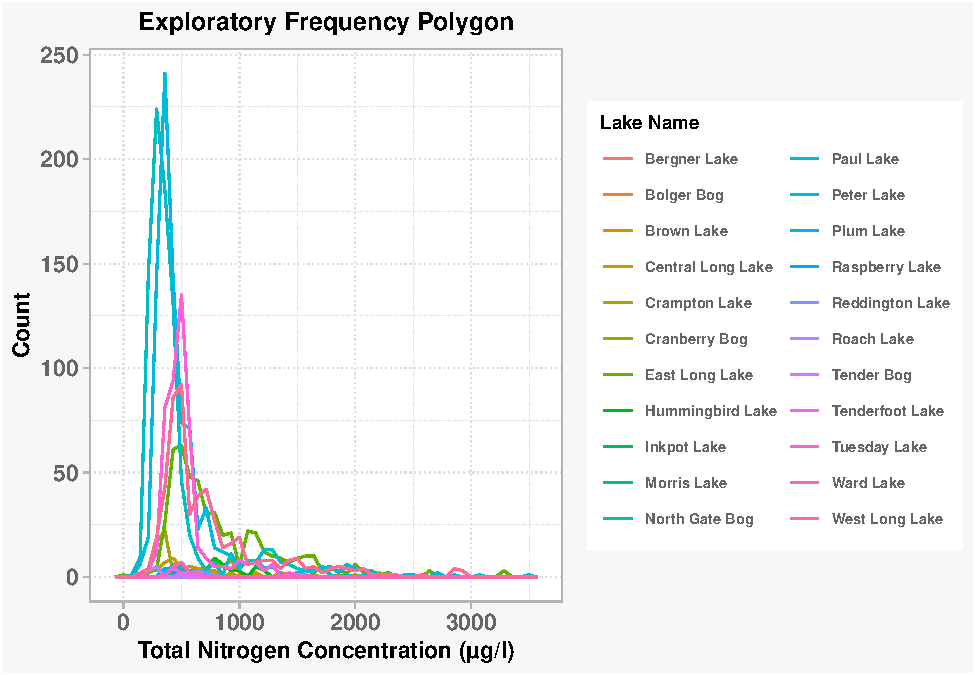
\includegraphics{Eadala_ENV872_Project_files/figure-latex/fig1-1.pdf}
\caption{Nitrogen concentration frequency polygon.}
\end{figure}

\begin{figure}
\centering
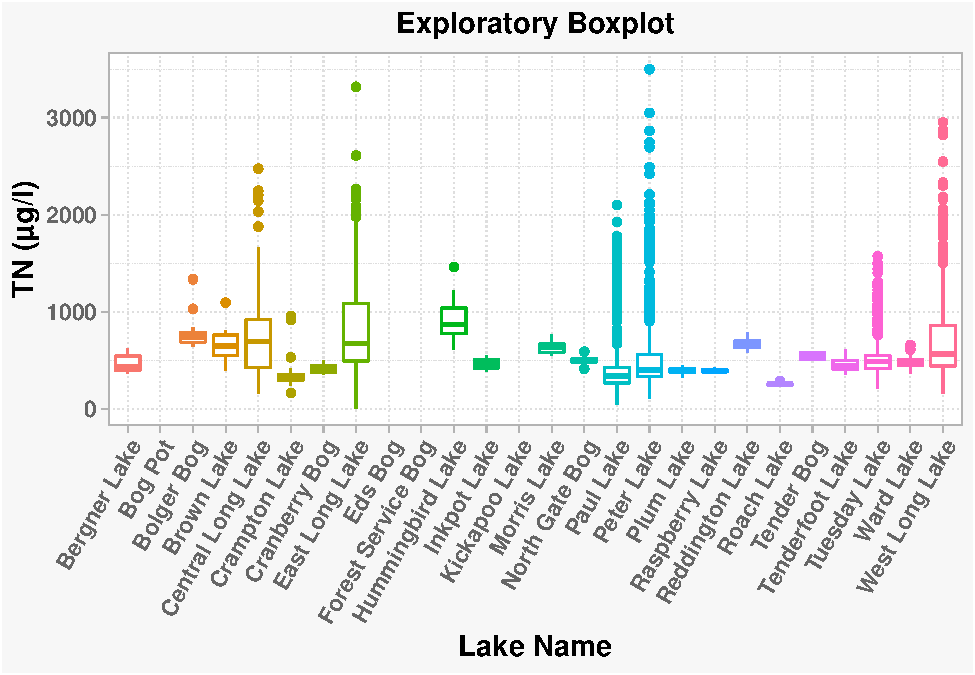
\includegraphics{Eadala_ENV872_Project_files/figure-latex/fig2-1.pdf}
\caption{Nitrogen concentration boxplot.}
\end{figure}

\begin{figure}
\centering
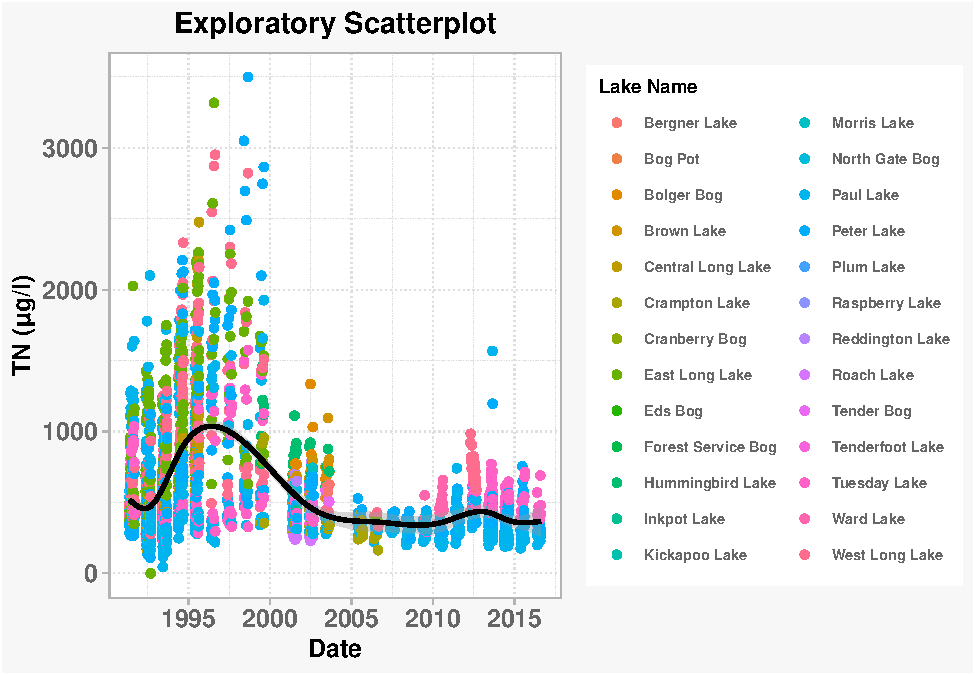
\includegraphics{Eadala_ENV872_Project_files/figure-latex/fig3-1.pdf}
\caption{Nitrogen concentration scatterplot.}
\end{figure}

Visual data exploration of the chemistry-physics data raw file in Figure
4.

\begin{figure}
\centering
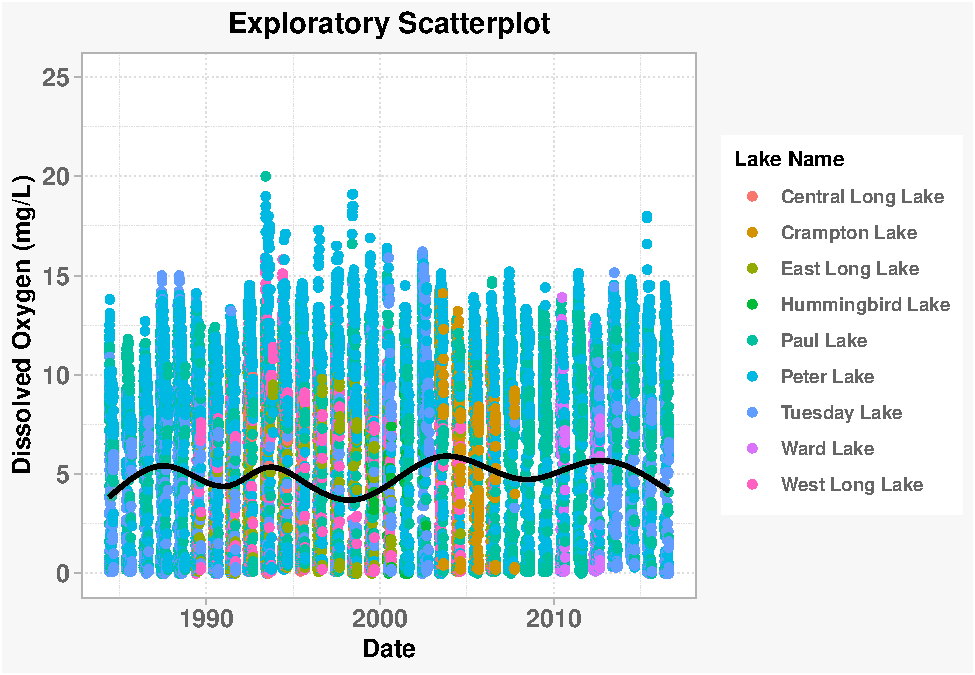
\includegraphics{Eadala_ENV872_Project_files/figure-latex/fig4-1.pdf}
\caption{Dissolved oxygen scatterplot.}
\end{figure}

Wrangling of data to include only the most meaningful variables and
compatible data for combining the two datasets.

\begin{Shaded}
\begin{Highlighting}[]
\CommentTok{# Find out what years are included in the chemistry-physics dataset}
\KeywordTok{list}\NormalTok{(}\KeywordTok{unique}\NormalTok{(ChemistryPhysics_raw}\OperatorTok{$}\NormalTok{year4))}
\end{Highlighting}
\end{Shaded}

\begin{verbatim}
## [[1]]
##  [1] 1984 1985 1986 1987 1988 1989 1990 1991 1992 1993 1994 1995 1996 1997 1998
## [16] 1999 2000 2001 2002 2003 2004 2005 2006 2007 2008 2009 2010 2011 2012 2013
## [31] 2014 2015 2016
\end{verbatim}

\begin{Shaded}
\begin{Highlighting}[]
\CommentTok{# Find out what years are included in the Nutrients dataset}
\KeywordTok{list}\NormalTok{(}\KeywordTok{unique}\NormalTok{(Nutrients_raw}\OperatorTok{$}\NormalTok{year4))}
\end{Highlighting}
\end{Shaded}

\begin{verbatim}
## [[1]]
##  [1] 1991 1992 1993 1994 1995 1996 1997 1998 1999 2000 2001 2002 2003 2005 2006
## [16] 2007 2008 2009 2010 2011 2012 2013 2014 2015 2016
\end{verbatim}

\begin{Shaded}
\begin{Highlighting}[]
\CommentTok{# Keep only useful columns to minimize the number of NAs later and filter only the years that are common to both datasets}
\NormalTok{Nutrients_processed <-}\StringTok{ }\NormalTok{Nutrients_raw }\OperatorTok
\StringTok{  }\KeywordTok{select}\NormalTok{(}\OperatorTok{-}\NormalTok{lakeid, }\OperatorTok{-}\NormalTok{depth_id , }\OperatorTok{-}\NormalTok{nh34, }\OperatorTok{-}\NormalTok{no23, }\OperatorTok{-}\NormalTok{po4, }\OperatorTok{-}\NormalTok{comments) }\OperatorTok
\StringTok{  }\KeywordTok{filter}\NormalTok{(year4 }\OperatorTok{==}\StringTok{ }\DecValTok{1991} \OperatorTok{|}\StringTok{ }\NormalTok{year4 }\OperatorTok{==}\StringTok{ }\DecValTok{1992} \OperatorTok{|}\StringTok{ }\NormalTok{year4 }\OperatorTok{==}\StringTok{  }\DecValTok{1993} \OperatorTok{|}\StringTok{ }\NormalTok{year4 }\OperatorTok{==}\StringTok{  }\DecValTok{1994} \OperatorTok{|}\StringTok{ }\NormalTok{year4 }\OperatorTok{==}\StringTok{ }\DecValTok{1999} \OperatorTok{|}\StringTok{ }\NormalTok{year4 }\OperatorTok{==}\StringTok{  }\DecValTok{2000} \OperatorTok{|}\StringTok{ }\NormalTok{year4 }\OperatorTok{==}\StringTok{ }\DecValTok{2001} \OperatorTok{|}\StringTok{ }\NormalTok{year4 }\OperatorTok{==}\StringTok{ }\DecValTok{2002} \OperatorTok{|}\StringTok{ }\NormalTok{year4 }\OperatorTok{==}\StringTok{ }\DecValTok{2003} \OperatorTok{|}\StringTok{ }\NormalTok{year4 }\OperatorTok{==}\StringTok{ }\DecValTok{2005} \OperatorTok{|}\StringTok{ }\NormalTok{year4 }\OperatorTok{==}\StringTok{  }\DecValTok{2006} \OperatorTok{|}\StringTok{ }\NormalTok{year4 }\OperatorTok{==}\StringTok{ }\DecValTok{2007}\OperatorTok{|}\StringTok{ }\NormalTok{year4 }\OperatorTok{==}\StringTok{ }\DecValTok{2008} \OperatorTok{|}\StringTok{ }\NormalTok{year4 }\OperatorTok{==}\StringTok{ }\DecValTok{2009} \OperatorTok{|}\StringTok{ }\NormalTok{year4 }\OperatorTok{==}\StringTok{ }\DecValTok{2010} \OperatorTok{|}\StringTok{ }\NormalTok{year4 }\OperatorTok{==}\StringTok{  }\DecValTok{2011} \OperatorTok{|}\StringTok{ }\NormalTok{year4 }\OperatorTok{==}\StringTok{  }\DecValTok{2012} \OperatorTok{|}\StringTok{ }\NormalTok{year4 }\OperatorTok{==}\StringTok{  }\DecValTok{2013} \OperatorTok{|}\StringTok{ }\NormalTok{year4 }\OperatorTok{==}\StringTok{  }\DecValTok{2014} \OperatorTok{|}\StringTok{ }\NormalTok{year4 }\OperatorTok{==}\StringTok{ }\DecValTok{2015} \OperatorTok{|}\StringTok{ }\NormalTok{year4 }\OperatorTok{==}\StringTok{ }\DecValTok{2016}\NormalTok{) }

\CommentTok{# Keep only useful columns to minimize the number of NAs later and filter only the years that are common to both datasets}
\NormalTok{ChemistryPhysics_processed <-}\StringTok{ }\NormalTok{ChemistryPhysics_raw }\OperatorTok
\StringTok{  }\KeywordTok{select}\NormalTok{(}\OperatorTok{-}\NormalTok{lakeid, }\OperatorTok{-}\NormalTok{irradianceDeck, }\OperatorTok{-}\NormalTok{irradianceWater, }\OperatorTok{-}\NormalTok{comments) }\OperatorTok\StringTok{ }
\StringTok{  }\KeywordTok{filter}\NormalTok{(year4 }\OperatorTok{==}\StringTok{ }\DecValTok{1991} \OperatorTok{|}\StringTok{ }\NormalTok{year4 }\OperatorTok{==}\StringTok{ }\DecValTok{1992} \OperatorTok{|}\StringTok{ }\NormalTok{year4 }\OperatorTok{==}\StringTok{  }\DecValTok{1993} \OperatorTok{|}\StringTok{ }\NormalTok{year4 }\OperatorTok{==}\StringTok{  }\DecValTok{1994} \OperatorTok{|}\StringTok{ }\NormalTok{year4 }\OperatorTok{==}\StringTok{ }\DecValTok{1999} \OperatorTok{|}\StringTok{ }\NormalTok{year4 }\OperatorTok{==}\StringTok{  }\DecValTok{2000} \OperatorTok{|}\StringTok{ }\NormalTok{year4 }\OperatorTok{==}\StringTok{ }\DecValTok{2001} \OperatorTok{|}\StringTok{ }\NormalTok{year4 }\OperatorTok{==}\StringTok{ }\DecValTok{2002} \OperatorTok{|}\StringTok{ }\NormalTok{year4 }\OperatorTok{==}\StringTok{ }\DecValTok{2003} \OperatorTok{|}\StringTok{ }\NormalTok{year4 }\OperatorTok{==}\StringTok{ }\DecValTok{2005} \OperatorTok{|}\StringTok{ }\NormalTok{year4 }\OperatorTok{==}\StringTok{  }\DecValTok{2006} \OperatorTok{|}\StringTok{ }\NormalTok{year4 }\OperatorTok{==}\StringTok{ }\DecValTok{2007}\OperatorTok{|}\StringTok{ }\NormalTok{year4 }\OperatorTok{==}\StringTok{ }\DecValTok{2008} \OperatorTok{|}\StringTok{ }\NormalTok{year4 }\OperatorTok{==}\StringTok{ }\DecValTok{2009} \OperatorTok{|}\StringTok{ }\NormalTok{year4 }\OperatorTok{==}\StringTok{ }\DecValTok{2010} \OperatorTok{|}\StringTok{ }\NormalTok{year4 }\OperatorTok{==}\StringTok{  }\DecValTok{2011} \OperatorTok{|}\StringTok{ }\NormalTok{year4 }\OperatorTok{==}\StringTok{  }\DecValTok{2012} \OperatorTok{|}\StringTok{ }\NormalTok{year4 }\OperatorTok{==}\StringTok{  }\DecValTok{2013} \OperatorTok{|}\StringTok{ }\NormalTok{year4 }\OperatorTok{==}\StringTok{  }\DecValTok{2014} \OperatorTok{|}\StringTok{ }\NormalTok{year4 }\OperatorTok{==}\StringTok{ }\DecValTok{2015} \OperatorTok{|}\StringTok{ }\NormalTok{year4 }\OperatorTok{==}\StringTok{ }\DecValTok{2016}\NormalTok{)}

\CommentTok{# List the unique lake names in the processed nutrients dataset}
\KeywordTok{list}\NormalTok{(}\KeywordTok{unique}\NormalTok{(Nutrients_processed}\OperatorTok{$}\NormalTok{lakename))}
\end{Highlighting}
\end{Shaded}

\begin{verbatim}
## [[1]]
##  [1] Paul Lake          Peter Lake         East Long Lake     West Long Lake    
##  [5] Tuesday Lake       Central Long Lake  Hummingbird Lake   Crampton Lake     
##  [9] Brown Lake         Bergner Lake       Bolger Bog         Bog Pot           
## [13] Cranberry Bog      Eds Bog            Forest Service Bog Inkpot Lake       
## [17] Kickapoo Lake      Morris Lake        North Gate Bog     Plum Lake         
## [21] Raspberry Lake     Reddington Lake    Roach Lake         Tenderfoot Lake   
## [25] Ward Lake          Tender Bog        
## 26 Levels: Bergner Lake Bog Pot Bolger Bog Brown Lake ... West Long Lake
\end{verbatim}

\begin{Shaded}
\begin{Highlighting}[]
\CommentTok{# List the unique lake names in the processed chemistry-physics dataset}
\KeywordTok{list}\NormalTok{(}\KeywordTok{unique}\NormalTok{(ChemistryPhysics_processed}\OperatorTok{$}\NormalTok{lakename))}
\end{Highlighting}
\end{Shaded}

\begin{verbatim}
## [[1]]
## [1] Paul Lake         Peter Lake        East Long Lake    West Long Lake   
## [5] Tuesday Lake      Central Long Lake Hummingbird Lake  Crampton Lake    
## [9] Ward Lake        
## 9 Levels: Central Long Lake Crampton Lake East Long Lake ... West Long Lake
\end{verbatim}

\begin{Shaded}
\begin{Highlighting}[]
\CommentTok{# Combine the two datasets and filter only the common and interested lakes from the two datasets}
\NormalTok{Combined_processed <-}\StringTok{ }\KeywordTok{full_join}\NormalTok{(Nutrients_processed, ChemistryPhysics_processed) }\OperatorTok
\StringTok{  }\KeywordTok{filter}\NormalTok{(year4 }\OperatorTok{==}\StringTok{ }\DecValTok{1991} \OperatorTok{|}\StringTok{ }\NormalTok{year4 }\OperatorTok{==}\StringTok{ }\DecValTok{1992} \OperatorTok{|}\StringTok{ }\NormalTok{year4 }\OperatorTok{==}\StringTok{  }\DecValTok{1993} \OperatorTok{|}\StringTok{ }\NormalTok{year4 }\OperatorTok{==}\StringTok{  }\DecValTok{1994} \OperatorTok{|}\StringTok{ }\NormalTok{year4 }\OperatorTok{==}\StringTok{ }\DecValTok{1999} \OperatorTok{|}\StringTok{ }\NormalTok{year4 }\OperatorTok{==}\StringTok{  }\DecValTok{2000} \OperatorTok{|}\StringTok{ }\NormalTok{year4 }\OperatorTok{==}\StringTok{ }\DecValTok{2001} \OperatorTok{|}\StringTok{ }\NormalTok{year4 }\OperatorTok{==}\StringTok{ }\DecValTok{2002} \OperatorTok{|}\StringTok{ }\NormalTok{year4 }\OperatorTok{==}\StringTok{ }\DecValTok{2003} \OperatorTok{|}\StringTok{ }\NormalTok{year4 }\OperatorTok{==}\StringTok{ }\DecValTok{2005} \OperatorTok{|}\StringTok{ }\NormalTok{year4 }\OperatorTok{==}\StringTok{  }\DecValTok{2006} \OperatorTok{|}\StringTok{ }\NormalTok{year4 }\OperatorTok{==}\StringTok{ }\DecValTok{2007}\OperatorTok{|}\StringTok{ }\NormalTok{year4 }\OperatorTok{==}\StringTok{ }\DecValTok{2008} \OperatorTok{|}\StringTok{ }\NormalTok{year4 }\OperatorTok{==}\StringTok{ }\DecValTok{2009} \OperatorTok{|}\StringTok{ }\NormalTok{year4 }\OperatorTok{==}\StringTok{ }\DecValTok{2010} \OperatorTok{|}\StringTok{ }\NormalTok{year4 }\OperatorTok{==}\StringTok{  }\DecValTok{2011} \OperatorTok{|}\StringTok{ }\NormalTok{year4 }\OperatorTok{==}\StringTok{  }\DecValTok{2012} \OperatorTok{|}\StringTok{ }\NormalTok{year4 }\OperatorTok{==}\StringTok{  }\DecValTok{2013} \OperatorTok{|}\StringTok{ }\NormalTok{year4 }\OperatorTok{==}\StringTok{  }\DecValTok{2014} \OperatorTok{|}\StringTok{ }\NormalTok{year4 }\OperatorTok{==}\StringTok{ }\DecValTok{2015} \OperatorTok{|}\StringTok{ }\NormalTok{year4 }\OperatorTok{==}\StringTok{ }\DecValTok{2016}\NormalTok{) }\OperatorTok
\StringTok{  }\KeywordTok{filter}\NormalTok{(lakename }\OperatorTok{==}\StringTok{ "Paul Lake"} \OperatorTok{|}\StringTok{ }\NormalTok{lakename }\OperatorTok{==}\StringTok{ "Peter Lake"} \OperatorTok{|}\StringTok{ }\NormalTok{lakename }\OperatorTok{==}\StringTok{ "East Long Lake"} \OperatorTok{|}\StringTok{ }\NormalTok{lakename }\OperatorTok{==}\StringTok{ "West Long Lake"} \OperatorTok{|}\StringTok{ }\NormalTok{lakename }\OperatorTok{==}\StringTok{ "Tuesday Lake"} \OperatorTok{|}\StringTok{ }\NormalTok{lakename }\OperatorTok{==}\StringTok{ "Crampton Lake"}\NormalTok{)}

\CommentTok{# Save the combined data in the processed folder}
\KeywordTok{write.csv}\NormalTok{(Combined_processed, }\DataTypeTok{row.names =} \OtherTok{FALSE}\NormalTok{, }\DataTypeTok{file =} \StringTok{"./Data/Processed/Combined_processed.csv"}\NormalTok{)}
\end{Highlighting}
\end{Shaded}

A Redfield ratio N:P of 16:1 by moles in general indicates a roughly
balanced supply of N and P, and algae assemblages tend to mirror this
ratio fairly closely when growing under balanced growth conditions
(\url{https://www.sciencedirect.com/topics/earth-and-planetary-sciences/redfield-ratio}).
Converting the molar ratio to migrogram ratio gives us N:P of 7.24:1,
since 1 mole of N = 14.0067g and 1 mole of P = 30.973761g
(\url{https://www.convertunits.com/from/grams+Nitrogen/to/moles};
\url{https://www.convertunits.com/from/grams+Phosphorus/to/moles})

First question for further data exploring: \emph{Are the lakes
phosphorus or nitrogen deficient?}

\begin{Shaded}
\begin{Highlighting}[]
\CommentTok{#To exlude some of the valariables from the dataset so that the number of NAs in the dataset could be minimized}
\NormalTok{NitrogenPhosphorus <-}\StringTok{ }\NormalTok{Combined_processed }\OperatorTok
\StringTok{  }\KeywordTok{select}\NormalTok{(}\OperatorTok{-}\NormalTok{temperature_C) }\OperatorTok
\StringTok{  }\KeywordTok{na.exclude}\NormalTok{()}

\CommentTok{# Save the new folder}
\KeywordTok{write.csv}\NormalTok{(NitrogenPhosphorus, }\DataTypeTok{row.names =} \OtherTok{FALSE}\NormalTok{, }\DataTypeTok{file =} \StringTok{"./Data/Processed/NitrogenPhosphorus_processed.csv"}\NormalTok{)}
\end{Highlighting}
\end{Shaded}

\emph{What is the average total nitrogen/total phosphorus (N:P) ratio
for each of the six north temperate lakes?}

\begin{Shaded}
\begin{Highlighting}[]
\NormalTok{NitrogenPhosphorus}\OperatorTok{$}\NormalTok{NPRatio <-}\StringTok{ }\NormalTok{NitrogenPhosphorus}\OperatorTok{$}\NormalTok{tn_ug }\OperatorTok{/}\StringTok{ }\NormalTok{NitrogenPhosphorus}\OperatorTok{$}\NormalTok{tp_ug }\CommentTok{# Gives us a new colum with the N:P ratio}

\CommentTok{# To summarize the N:P ratio in each lake }
\NormalTok{NPRatio.summary <-}\StringTok{ }\NormalTok{NitrogenPhosphorus }\OperatorTok
\StringTok{   }\KeywordTok{group_by}\NormalTok{(lakename) }\OperatorTok
\StringTok{  }\KeywordTok{summarise}\NormalTok{(}\DataTypeTok{mean.NPRatio =} \KeywordTok{mean}\NormalTok{(NPRatio, }\DataTypeTok{na.rm =} \OtherTok{TRUE}\NormalTok{),}
            \DataTypeTok{minimum.NPRatio =} \KeywordTok{min}\NormalTok{(NPRatio, }\DataTypeTok{na.rm =} \OtherTok{TRUE}\NormalTok{),}
            \DataTypeTok{maximum.NPRatio =} \KeywordTok{max}\NormalTok{(NPRatio, }\DataTypeTok{na.rm =} \OtherTok{TRUE}\NormalTok{),}
            \DataTypeTok{Standard.dev.NPRatio =} \KeywordTok{sd}\NormalTok{(NPRatio, }\DataTypeTok{na.rm =} \OtherTok{TRUE}\NormalTok{)) }\CommentTok{# Gives us summary stats of each of the lakes with respect to N:P}
\end{Highlighting}
\end{Shaded}

Figure 5 offers a visual to understand if most of the lakes are above or
below the Redfield Ratio. In other words, to understand if most of the
lakes are phosphorus or nitrogen limited.

Dashed line indicates the Redfield Ratio of 7.24:1, which indicates
optimal conditions for phytoplankton growth. The lakes above the
Redfield Ratio would be phosphorus limited while those below it would be
nitrogen limited.

\begin{figure}
\centering
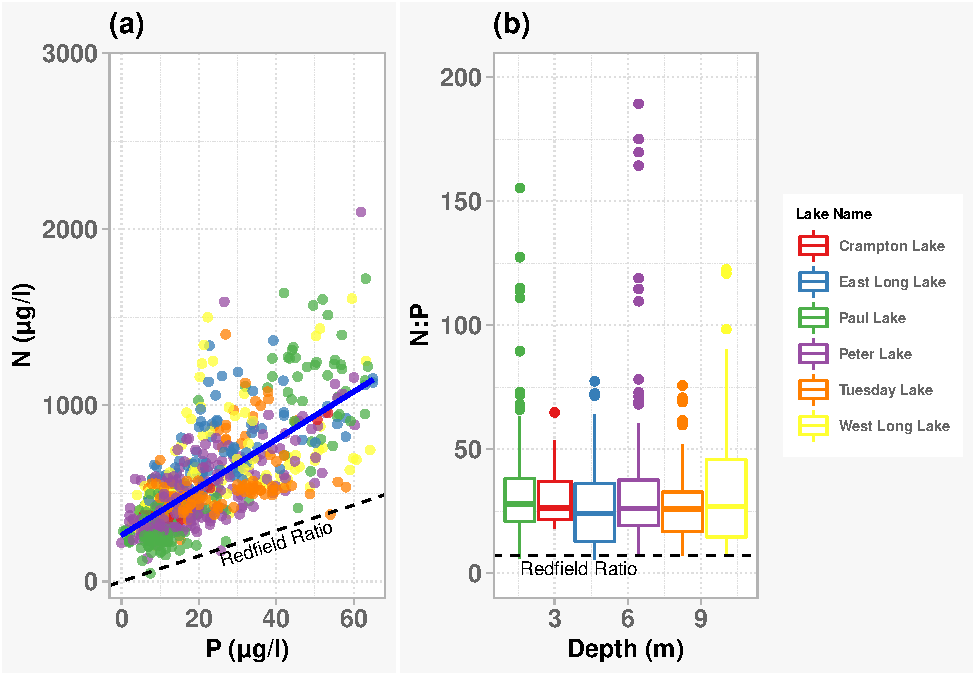
\includegraphics{Eadala_ENV872_Project_files/figure-latex/fig5-1.pdf}
\caption{(a) Nitrogen vs phosphorus concentration (b) Distribution of
N:P Ratio.}
\end{figure}

Figure 5 Tells us that most of the Lakes are phosphorus deficient,
therefore phosphorus should be the limiting nutrient prioritized or
addressed during water management.

\newpage

\hypertarget{analysis}{%
\section{Analysis}\label{analysis}}

\hypertarget{question-1-have-the-lakes-been-within-the-limiting-nutrient-criteria-over-the-years-how-does-the-np-ratio-impact-the-dissolved-oxygen-in-the-lakes}{%
\subsection{Question 1: Have the lakes been within the limiting nutrient
criteria over the years? How does the N:P ratio impact the dissolved
oxygen in the
lakes?}\label{question-1-have-the-lakes-been-within-the-limiting-nutrient-criteria-over-the-years-how-does-the-np-ratio-impact-the-dissolved-oxygen-in-the-lakes}}

\emph{One-sample t-test}

The figures under exploratory analysis tell us that all the eight lakes
are phosphorus deficient, and therefore phosphorus is the element that
needs to be controlled on priority to avoid eutrophication. EPA has
compiled state, territorial, and authorized tribal water quality
standards that EPA has approved or are otherwise in effect for Clean
Water Act purposes. According to this compilation, Wisconsin's
stratified lakes' total phosphorus criterion is not more than 30µg/l
(\url{https://www.epa.gov/wqs-tech/state-specific-water-quality-standards-effective-under-clean-water-act-cwa\#tb2}).
According to Carlson R.E. and J. Simpson in 1996, phosphorus
concentration between 24µg/l and 96µg/l suggests eutrophic conditions,
and anything above 96µg/l suggests hypereutrophic conditions
(\url{https://en.wikipedia.org/wiki/Trophic_state_index}). Therefore, it
is important to check if the eight North Temperate Lakes are at least
within the 30µg/l criterion or not.

This statistical analysis will test the null hypothesis that the means
of the total phosphorus concentrations in the eight North Temperate
Lakes are below the regulatory standard of 30µg/l.

First, the assumption of normal distribution is evaluated through the
Shapiro-Wilk normality test.

\begin{Shaded}
\begin{Highlighting}[]
\KeywordTok{shapiro.test}\NormalTok{(NitrogenPhosphorus}\OperatorTok{$}\NormalTok{tp_ug)}
\end{Highlighting}
\end{Shaded}

\begin{verbatim}
## 
##  Shapiro-Wilk normality test
## 
## data:  NitrogenPhosphorus$tp_ug
## W = 0.69337, p-value < 2.2e-16
\end{verbatim}

The Shapiro-Wilk normality test says that the total phosphorus
concentrations data in the six lakes of Wisconsin are significantly
different from a normal distribution (Shapiro-Wilk normality test; W =
0.69337, p-value \textless{} 0.0001)

Next, a visual analysis of the data is performed.

\begin{Shaded}
\begin{Highlighting}[]
\KeywordTok{hist}\NormalTok{(NitrogenPhosphorus}\OperatorTok{$}\NormalTok{tp_ug, }\DataTypeTok{breaks =} \DecValTok{50}\NormalTok{) }\CommentTok{# Phosphorus concentration histogram}
\end{Highlighting}
\end{Shaded}

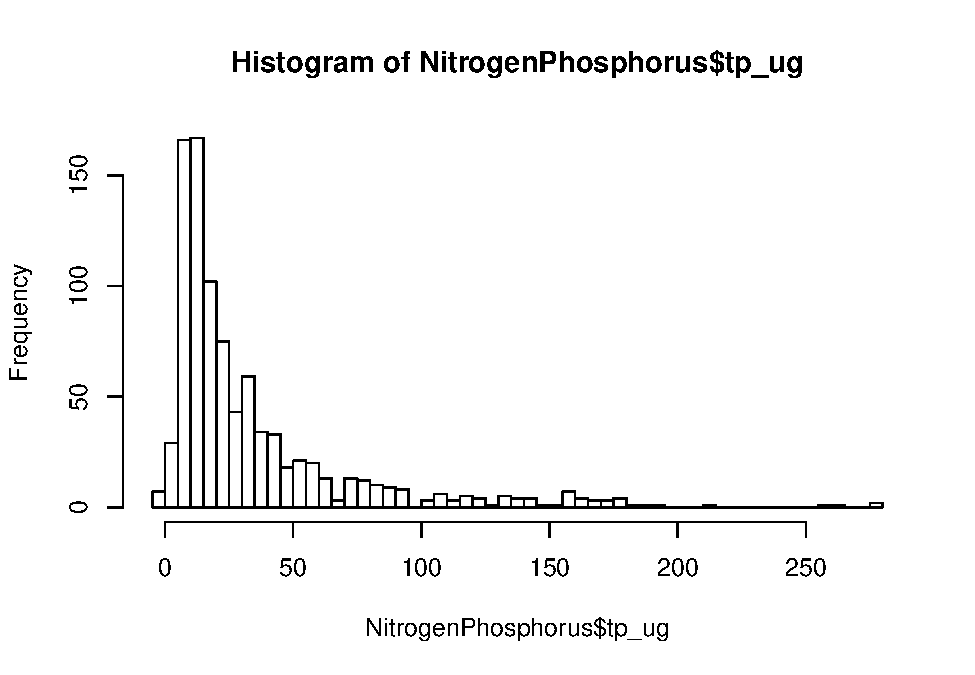
\includegraphics{Eadala_ENV872_Project_files/figure-latex/unnamed-chunk-9-1.pdf}

\begin{Shaded}
\begin{Highlighting}[]
\KeywordTok{qqnorm}\NormalTok{(NitrogenPhosphorus}\OperatorTok{$}\NormalTok{tp_ug, }\DataTypeTok{pch =} \DecValTok{1}\NormalTok{, }\DataTypeTok{frame =} \OtherTok{FALSE}\NormalTok{)}
\KeywordTok{qqline}\NormalTok{(NitrogenPhosphorus}\OperatorTok{$}\NormalTok{tp_ug, }\DataTypeTok{col =} \StringTok{"blue"}\NormalTok{, }\DataTypeTok{lwd =} \DecValTok{2}\NormalTok{)}
\end{Highlighting}
\end{Shaded}

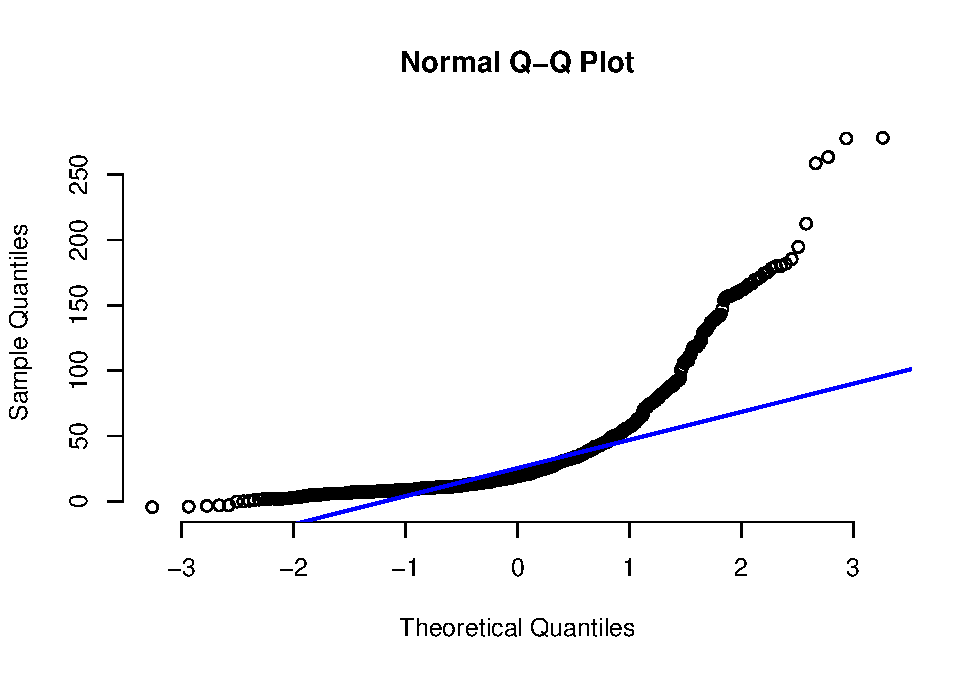
\includegraphics{Eadala_ENV872_Project_files/figure-latex/unnamed-chunk-9-2.pdf}

In the above figures it can be seen that the data distribution is
right-skewed with a longer tail to the right than a normal distribution;
nevertheless, environmental data often violate the assumptions of
normality and since the sample size is large, a t-test is performed
anyway.

\begin{Shaded}
\begin{Highlighting}[]
\KeywordTok{t.test}\NormalTok{(NitrogenPhosphorus}\OperatorTok{$}\NormalTok{tp_ug, }\DataTypeTok{mu =} \DecValTok{30}\NormalTok{, }\DataTypeTok{alternative =} \StringTok{"less"}\NormalTok{)}
\end{Highlighting}
\end{Shaded}

\begin{verbatim}
## 
##  One Sample t-test
## 
## data:  NitrogenPhosphorus$tp_ug
## t = 3.2053, df = 907, p-value = 0.9993
## alternative hypothesis: true mean is less than 30
## 95 percent confidence interval:
##      -Inf 36.36745
## sample estimates:
## mean of x 
##  34.20656
\end{verbatim}

According to the One Sample t-test, the TP concentrations for the North
Temperate Lakes of Wisconsin from 1991 to 2016 have not been
significantly lower than 30µg/l (one sample t-test; t = 3.2053, df =
907, p-value \textgreater{} 0.0001).

Figure 6 presents a visualization of the TP concentrations in Wisconsin
lakes data in comparison with the Wisconsin regulatory standard.

\begin{figure}
\centering
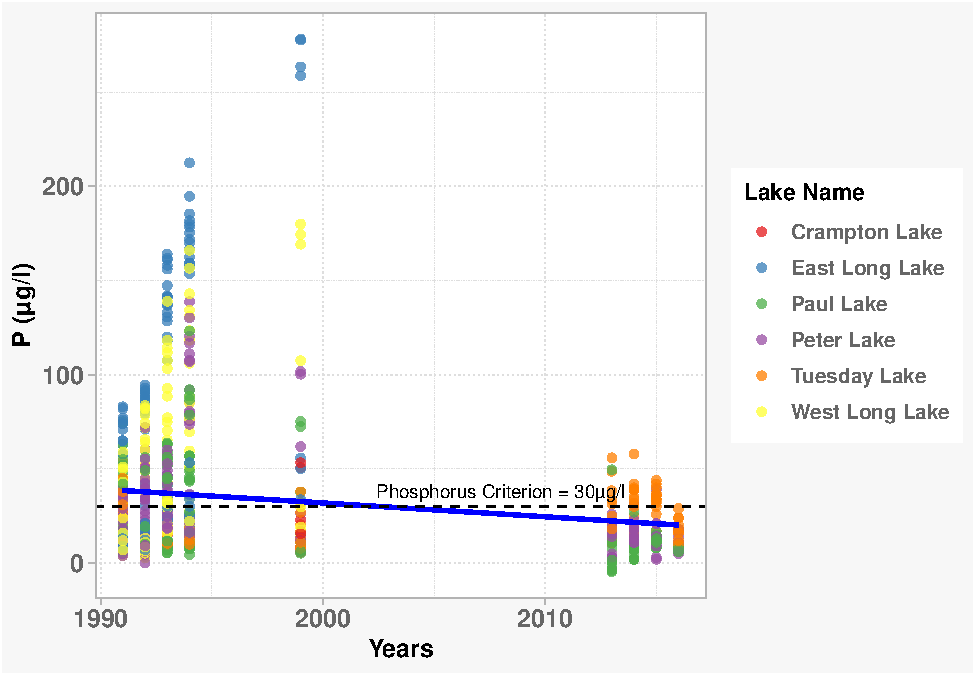
\includegraphics{Eadala_ENV872_Project_files/figure-latex/fig6-1.pdf}
\caption{Phosphorus concenration over years.}
\end{figure}

The blue line in comparison with the black dashed line indicates that
most of the Wisconsin lakes started off with phosphorus levels above the
criteria but have been able to lower their phosphorus in the most recent
recent years.

Coming the the next part of the research question, figure 7 gives us the
visual interpretation of how the N:P ratio affects the dissolved oxygen.

\begin{figure}
\centering
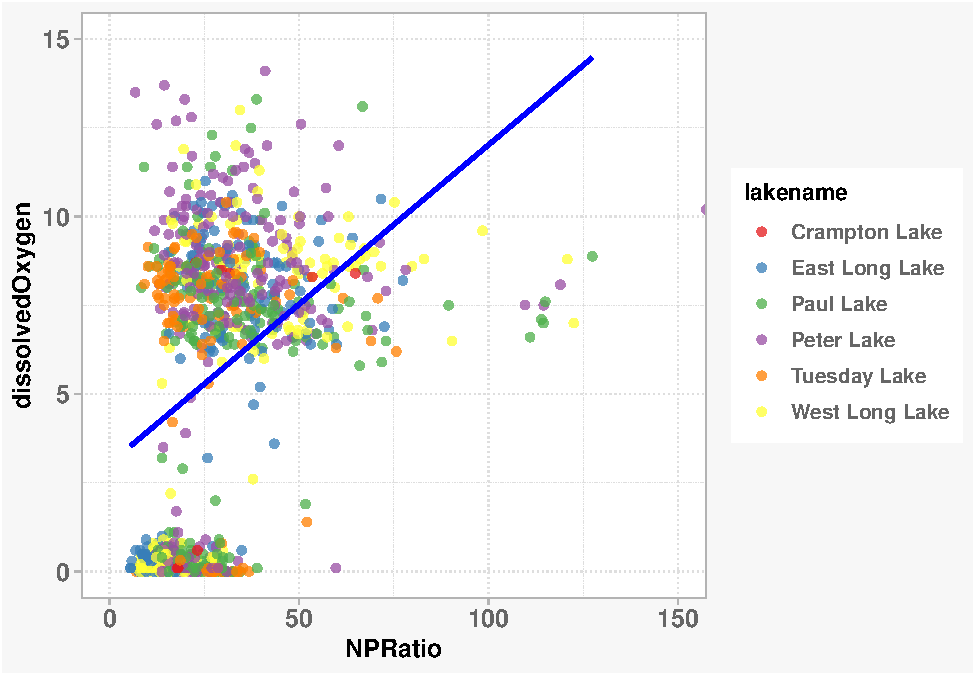
\includegraphics{Eadala_ENV872_Project_files/figure-latex/fig7-1.pdf}
\caption{Dissolved oxygen over N:P ratio}
\end{figure}

Figure 7 tells us that an increase in the N:P ratio increased dissolved
oxygen in the lakes. This is consistent with the theory that controlling
phosphorus concentration in phosphorus deficient lakes can can preserve
their water quality. However, phosphorus might not be the only factor
affecting the dissolved oxygen and eventually the water quality of
water. Therefore, it is important to understand what other variables
affect dissolved oxygen, whose depletion indicates eutrophication in
many cases.

\hypertarget{question-2-what-are-the-best-set-of-predictors-of-dissolved-oxygen-across-the-monitoring-period-at-the-north-temperate-lakes-lter}{%
\subsection{Question 2: What are the best set of predictors of dissolved
oxygen across the monitoring period at the North Temperate Lakes
LTER?}\label{question-2-what-are-the-best-set-of-predictors-of-dissolved-oxygen-across-the-monitoring-period-at-the-north-temperate-lakes-lter}}

\emph{Linear model}

To answer this question, a generalized linear model approach was taken.

Since multiple explanatory variables are being considered at a time in
the model, it is important to check the model is not over-parameterized.
Therefore, the Akaike's Information Criteria (AIC) was used.

\begin{Shaded}
\begin{Highlighting}[]
\NormalTok{DO.predictors <-}\StringTok{ }\NormalTok{Combined_processed }\OperatorTok
\StringTok{  }\KeywordTok{na.exclude}\NormalTok{()}

\NormalTok{DO.AIC <-}\StringTok{ }\KeywordTok{lm}\NormalTok{(}\DataTypeTok{data =}\NormalTok{ DO.predictors, dissolvedOxygen }\OperatorTok{~}\StringTok{ }\NormalTok{year4 }\OperatorTok{+}\StringTok{ }\NormalTok{daynum }\OperatorTok{+}\StringTok{ }\NormalTok{temperature_C }\OperatorTok{+}\StringTok{ }\NormalTok{tn_ug }\OperatorTok{+}\StringTok{ }\NormalTok{tp_ug }\OperatorTok{+}\StringTok{ }\NormalTok{depth) }\CommentTok{# Runs an AIC to determine what set of explanatory variables is best suited to predict dissolved oxygen}
\KeywordTok{step}\NormalTok{(DO.AIC) }\CommentTok{# The lower the AIC value, the better}
\end{Highlighting}
\end{Shaded}

\begin{verbatim}
## Start:  AIC=1015.33
## dissolvedOxygen ~ year4 + daynum + temperature_C + tn_ug + tp_ug + 
##     depth
## 
##                 Df Sum of Sq    RSS    AIC
## <none>                       2735.7 1015.3
## - tp_ug          1     25.85 2761.6 1021.9
## - year4          1     29.13 2764.9 1022.9
## - daynum         1     39.13 2774.9 1026.2
## - tn_ug          1    100.08 2835.8 1045.9
## - temperature_C  1    119.62 2855.3 1052.2
## - depth          1   2046.68 4782.4 1519.9
\end{verbatim}

\begin{verbatim}
## 
## Call:
## lm(formula = dissolvedOxygen ~ year4 + daynum + temperature_C + 
##     tn_ug + tp_ug + depth, data = DO.predictors)
## 
## Coefficients:
##   (Intercept)          year4         daynum  temperature_C          tn_ug  
##     59.781118      -0.023206      -0.006947      -0.137099      -0.001380  
##         tp_ug          depth  
##      0.007627      -0.874667
\end{verbatim}

The best predictors from the lowest AIC are: year, daynum,
temperature\_C, tn\_ug, tp\_ug and depth.

Next, a multiple regression is performed on the recommended set of
variables.

\begin{Shaded}
\begin{Highlighting}[]
\NormalTok{DO.model <-}\StringTok{ }\KeywordTok{lm}\NormalTok{(}\DataTypeTok{data =}\NormalTok{ DO.predictors, dissolvedOxygen }\OperatorTok{~}\StringTok{ }\NormalTok{year4 }\OperatorTok{+}\StringTok{ }\NormalTok{daynum }\OperatorTok{+}\StringTok{ }\NormalTok{temperature_C }\OperatorTok{+}\StringTok{ }\NormalTok{depth }\OperatorTok{+}\StringTok{ }\NormalTok{tn_ug }\OperatorTok{+}\StringTok{ }\NormalTok{tp_ug) }
\KeywordTok{anova}\NormalTok{(DO.model)}
\end{Highlighting}
\end{Shaded}

\begin{verbatim}
## Analysis of Variance Table
## 
## Response: dissolvedOxygen
##                Df Sum Sq Mean Sq  F value    Pr(>F)    
## year4           1  759.0   759.0  249.705 < 2.2e-16 ***
## daynum          1  275.3   275.3   90.573 < 2.2e-16 ***
## temperature_C   1 8357.3  8357.3 2749.378 < 2.2e-16 ***
## depth           1 2407.5  2407.5  792.007 < 2.2e-16 ***
## tn_ug           1   76.4    76.4   25.141 6.419e-07 ***
## tp_ug           1   25.8    25.8    8.503  0.003634 ** 
## Residuals     900 2735.7     3.0                       
## ---
## Signif. codes:  0 '***' 0.001 '**' 0.01 '*' 0.05 '.' 0.1 ' ' 1
\end{verbatim}

The full model also reconfirmed the above variables as the best. So
model is run with the same variables.

\begin{Shaded}
\begin{Highlighting}[]
\NormalTok{DO.model <-}\StringTok{ }\KeywordTok{lm}\NormalTok{(}\DataTypeTok{data =}\NormalTok{ DO.predictors, dissolvedOxygen }\OperatorTok{~}\StringTok{ }\NormalTok{year4 }\OperatorTok{+}\StringTok{ }\NormalTok{daynum }\OperatorTok{+}\StringTok{ }\NormalTok{temperature_C }\OperatorTok{+}\StringTok{ }\NormalTok{depth }\OperatorTok{+}\StringTok{ }\NormalTok{tn_ug }\OperatorTok{+}\StringTok{ }\NormalTok{tp_ug) }\CommentTok{# Asserts the chosen model}
\KeywordTok{summary}\NormalTok{(DO.model) }\CommentTok{# Runs a multiple regression on the above recommended set of variables}
\end{Highlighting}
\end{Shaded}

\begin{verbatim}
## 
## Call:
## lm(formula = dissolvedOxygen ~ year4 + daynum + temperature_C + 
##     depth + tn_ug + tp_ug, data = DO.predictors)
## 
## Residuals:
##     Min      1Q  Median      3Q     Max 
## -6.1484 -0.7931 -0.1172  0.5387 10.1439 
## 
## Coefficients:
##                 Estimate Std. Error t value Pr(>|t|)    
## (Intercept)   59.7811180 14.9185927   4.007 6.65e-05 ***
## year4         -0.0232059  0.0074958  -3.096 0.002023 ** 
## daynum        -0.0069474  0.0019362  -3.588 0.000351 ***
## temperature_C -0.1370994  0.0218550  -6.273 5.49e-10 ***
## depth         -0.8746669  0.0337079 -25.948  < 2e-16 ***
## tn_ug         -0.0013804  0.0002406  -5.738 1.31e-08 ***
## tp_ug          0.0076268  0.0026155   2.916 0.003634 ** 
## ---
## Signif. codes:  0 '***' 0.001 '**' 0.01 '*' 0.05 '.' 0.1 ' ' 1
## 
## Residual standard error: 1.743 on 900 degrees of freedom
## Multiple R-squared:  0.8131, Adjusted R-squared:  0.8118 
## F-statistic: 652.6 on 6 and 900 DF,  p-value: < 2.2e-16
\end{verbatim}

The final set of variables that best predict the dissolved oxygen across
a monitoring period are year, day number, temperature, depth, nitrogen
concentration and phosphorus concentration. This set of variables
explain 81\% of variance (Adjusted R-squared = 0.8118, p-value
\textless{} 0.001)

\begin{figure}
\centering
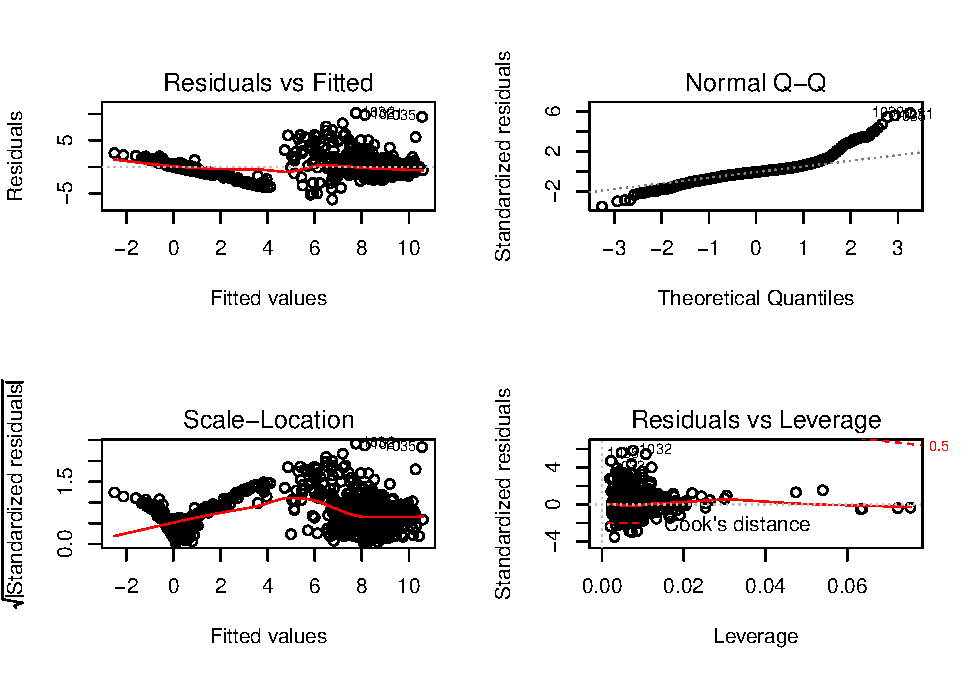
\includegraphics{Eadala_ENV872_Project_files/figure-latex/fig8-1.pdf}
\caption{Model diagnostic plots.}
\end{figure}

The following can be said about Figure 8:

\begin{enumerate}
\def\labelenumi{\arabic{enumi}.}
\item
  Residuals vs Fitted: Used to check the linear relationship
  assumptions. A horizontal line, without distinct patterns is an
  indication for a linear relationship; which is the case here.
\item
  Normal Q-Q: Used to examine whether the residuals are normally
  distributed. It's good if residuals points follow the straight dashed
  line. In this case the points do appear to follow an straight line
  (except for the extremes which is common for environmental data), so
  the graph is accepted.
\item
  Scale-Location (or Spread-Location): Used to check the homogeneity of
  variance of the residuals (homoscedasticity). Horizontal line with
  equally spread points is a good indication of homoscedasticity. In
  this case, the plot is difficult to predict so we can rely on the
  residual vs fitted data to assure homoscedasticity.
\item
  Residuals vs Leverage: Used to identify influential cases, that is
  extreme values that might influence the regression results when
  included or excluded from the analysis. In this case the outliers are
  not so influential that leaving them out might change the structure of
  the model.
\end{enumerate}

Given that our assumptions have been met, we can move on to the next
step. From the model we got that the intercept is 59.7811180, which is
the dissolved oxygen in mg/L, when all the other variables are zero.
Therefore, we reject the null hypothesis of no effect of the explanatory
variables on the response variable.

The year decreases the dissolved oxygen (mg/l) in the lakes
significantly. With an increase of 1 year, the dissolved oxygen is
decreased by 0.0232059 mg/l (t = -3.096, df = 900, p \textless{} 0.05).

The day number decreases the dissolved oxygen (mg/l) in the lakes highly
significantly. With an increase of 1 day, the dissolved oxygen is
decreased by 0.0069474 mg/l (t = -3.588, df = 900, p \textless{} 0.001).

The temperature decreases the dissolved oxygen (mg/l) in the lakes
highly significantly. With an increase in temperature by 1 Celsius, the
dissolved oxygen is decreased by 0.1370994 mg/l (t = -6.273, df = 900, p
\textless{} 0.001).

The depth decreases the dissolved oxygen (mg/l) in the lakes highly
significantly. With an increase in depth by 1 meter, the dissolved
oxygen is decreased by 0.8746669 mg/l (t = -25.948, df = 900, p
\textless{} 0.001).

The nitrogen concentration decreases the dissolved oxygen (mg/l) in the
lakes highly significantly. With an increase in nitrogen concentration
by 1 µg/l, the dissolved oxygen is decreased by 0.0013804 mg/l (t =
-5.738, df = 900, p \textless{} 0.001).

The phosphorus concentration increases the dissolved oxygen (mg/l) in
the lakes significantly. With an increase in phosphorus concentration by
1 µg/l, the dissolved oxygen is increased by 0.0076268 mg/l (t = 2.916,
df = 900, p \textless{} 0.05).

The final linear equation to predict dissolved oxygen (mg/l) from the
explanatory variables is:

\textbf{Dissolved oxygen in mg/l = 59.7811180 - 0.0232059xyear number -
0.0069474xday number - 0.1370994xtemperature in C - 0.8746669xdepth in m
- 0.0013804xTN in µg/l + 0.0076268xTP in µg/l}

Figure 9 - Figure 14 offer visual presentations of the dissolve oxygen
against each model variable.

\begin{figure}
\centering
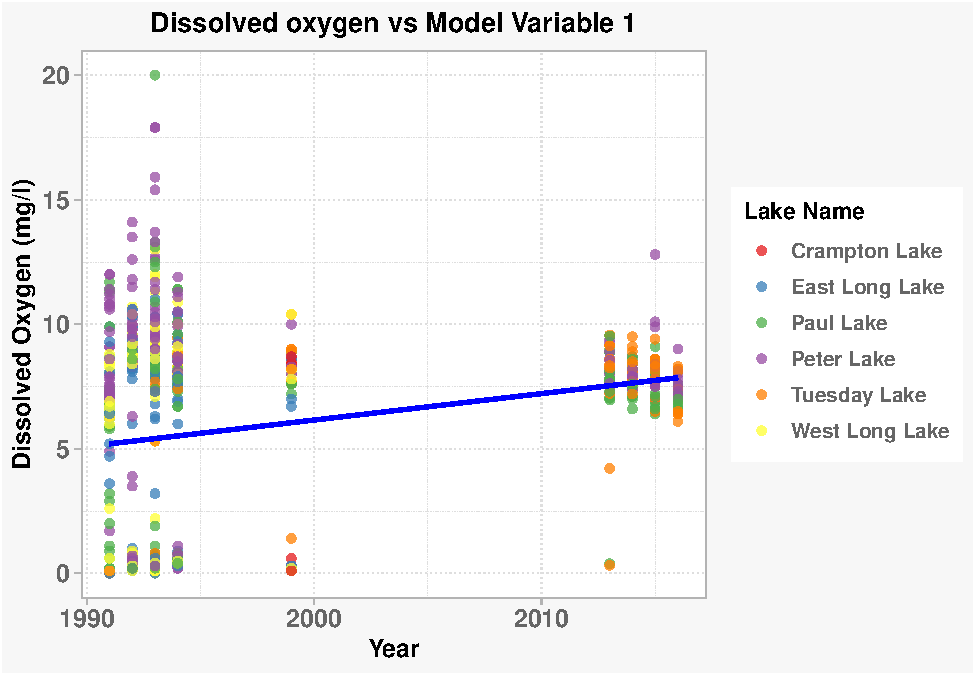
\includegraphics{Eadala_ENV872_Project_files/figure-latex/fig9-1.pdf}
\caption{Dissolved oxygen vs Years.}
\end{figure}

\begin{figure}
\centering
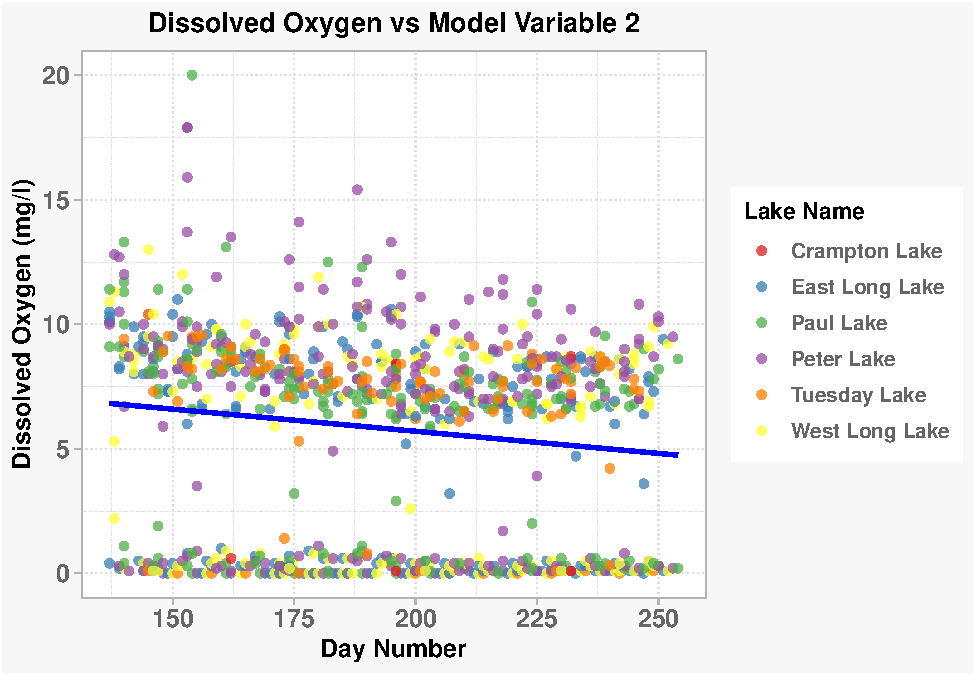
\includegraphics{Eadala_ENV872_Project_files/figure-latex/fig10-1.pdf}
\caption{Dissolved oxygen vs day number.}
\end{figure}

\begin{figure}
\centering
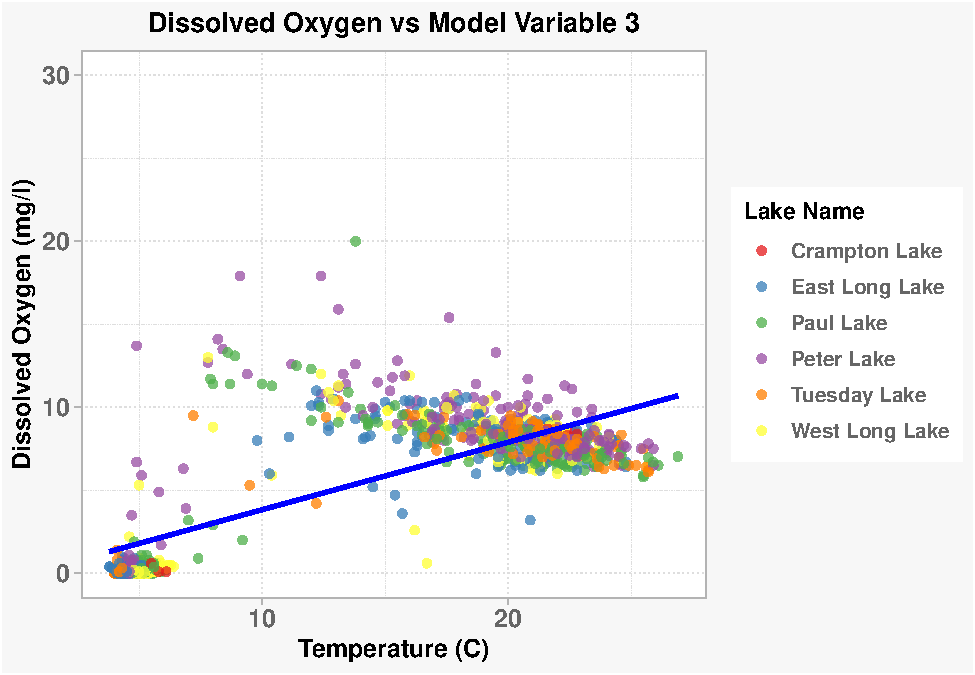
\includegraphics{Eadala_ENV872_Project_files/figure-latex/fig11-1.pdf}
\caption{Dissolved oxygen vs temperature.}
\end{figure}

\begin{figure}
\centering
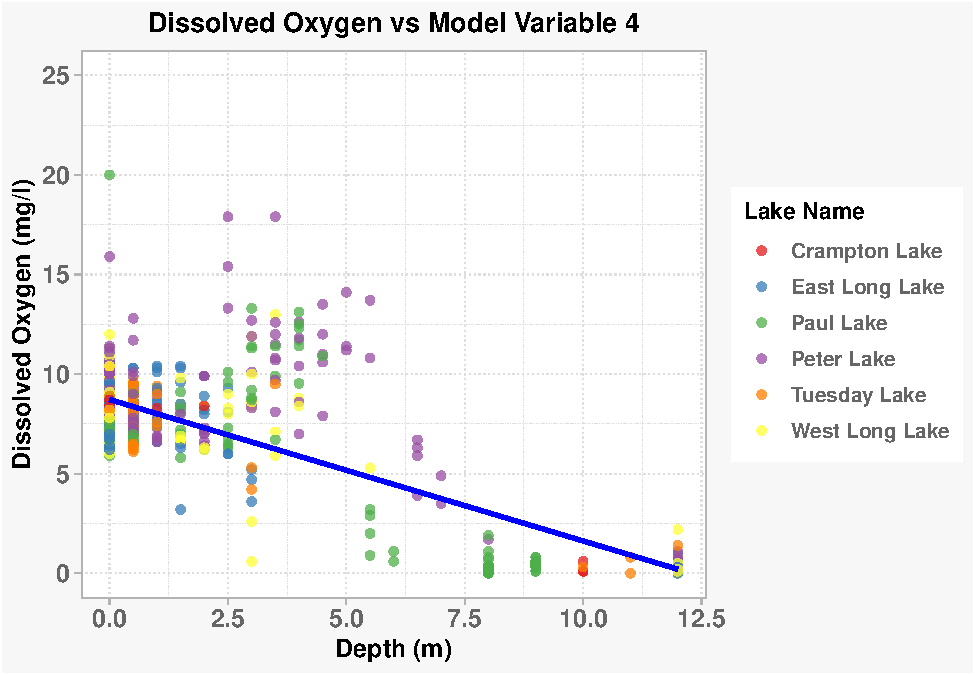
\includegraphics{Eadala_ENV872_Project_files/figure-latex/fig12-1.pdf}
\caption{Dissolved oxygen vs depth.}
\end{figure}

\begin{figure}
\centering
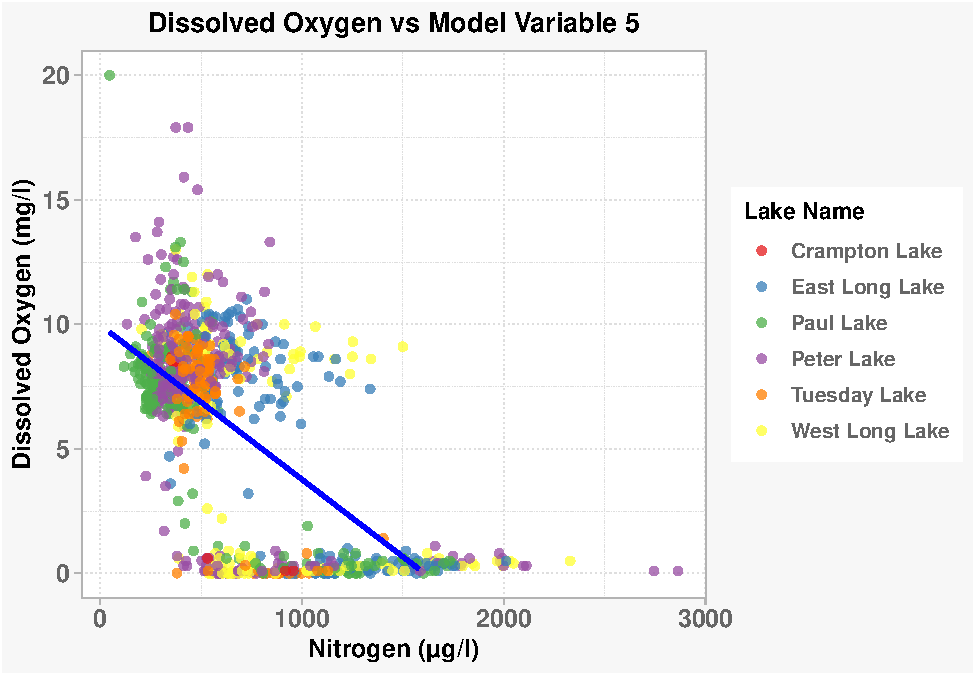
\includegraphics{Eadala_ENV872_Project_files/figure-latex/fig13-1.pdf}
\caption{Dissolved oxygen vs nitrogen concentration.}
\end{figure}

\begin{figure}
\centering
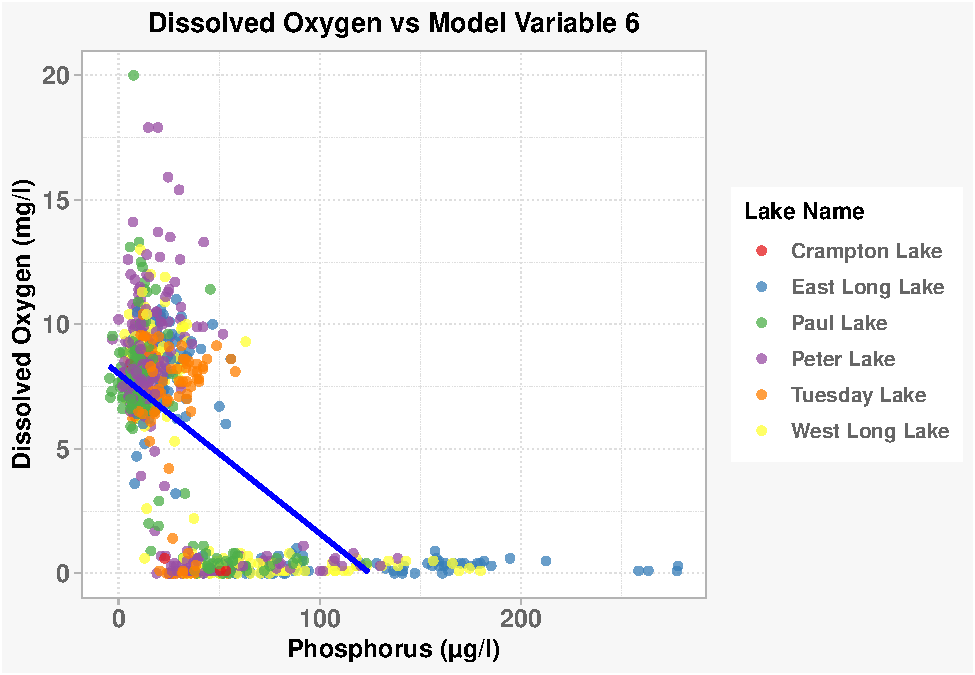
\includegraphics{Eadala_ENV872_Project_files/figure-latex/fig14-1.pdf}
\caption{Dissolved oxygen vs phosphorus concentration.}
\end{figure}

\newpage

\hypertarget{summary-and-conclusions}{%
\section{Summary and Conclusions}\label{summary-and-conclusions}}

I began this project with a set of exploratory questions that helped
arrive at the necessary data analysis methods to eventually answer the
the two research questions. Below are the key findings of this data
analysis project stemming from key questions asked during this entire
process (not just exclusive to the two main research questions or their
subsets):

\begin{enumerate}
\def\labelenumi{\arabic{enumi}.}
\item
  Majority of the lakes were found to be above the line of Redfield
  Ratio, therefore confirming that all the lakes in the dataset used
  were phosphorus deficient. This means that phosphorus can controlled
  to avoid eutrophication.
\item
  Most of the lakes were found to have a mean N:P ratio much above the
  Redfield Ratio. However, there have been instances of almost all of
  them having touched the Redfield Ratio.
\item
  The N:P ratio is found to be somewhat positively correlated to the
  dissolved oxygen in the lakes. However, the scatterplots show that
  that there is a huge spread of dissolved oxygen at especially below
  the ratio 50. This could mean that there are other stronger factors
  effecting dissolved oxygen
\item
  The the phosphorus concentration has decreased slowly but consistently
  over the years, possibly hinting at successful water quality
  management. Last decade has seen the phosphorus concentration
  controlled, below the set state criterion.
\end{enumerate}

Other than the above, a major finding is that year number (possibly
depicting environmental changes), day number (depicting seasonal
changes), temperature, depth, nitrogen concentration and phosphorus
concentration together are a good predictors of dissolved oxygen. The
multiple regression model highlights several trends: increase in the
year number, day number, temperature, depth and nitrogen concentration
decreases dissolved oxygen significantly while increase in phosphorus
concentration increases dissolved oxygen significantly. However, not all
the plots (that include their respective regression line) are consistent
with models results. For example, the Lm() line in the dissolved oxygen
over temperature graph shows that there is a positive correlation
between the tow when it is supposed to the other way around. This is not
true in the real world since cold water can hold more dissolved oxygen.
However, is it possible that depth has had a more major effect on this
trend in this graph. Similarly, even though the model predicts that
increase in phosphorus should increase dissolved oxygen, the graph shows
the opposite. Once again, it is probably because there are interacting
and mixed effects involved. Therefore, there is more scope for further
statistical testing and analysis to confirm some of these correlations.

\end{document}
